\documentclass[11pt,a4paper,openright]{memoir}

% font encoding
\usepackage[T1]{fontenc}

% better tables
\usepackage{multirow}
\usepackage{array}
\newcommand{\specialcell}[2][c]{%
  \begin{tabular}[#1]{@{}c@{}}#2\end{tabular}}

% being able to quote
\usepackage[threshold=1]{csquotes}

% being able to cite code
\usepackage{verbatim}

% being able to use images
\usepackage{graphicx}

% columns hyphenation spacing
\usepackage{soul}
\usepackage{multicol}
\usepackage[document]{ragged2e}

% bibtex
\usepackage[backend=bibtex,bibencoding=ascii]{biblatex}
\usepackage{url}

% tables and NLP
% \usepackage{tikz} 
\usepackage{tikz-qtree}
\usepackage{tikz-dependency}

% graphs
\usepackage{pgfplots}
\pgfplotsset{compat=1.12}

% use xml
\usepackage{listings}

% This one includes babel in Australian mode
\usepackage{unswcover} 

% For the algorithm
\usepackage{algorithm}% http://ctan.org/pkg/algorithms
\usepackage{algpseudocode}% http://ctan.org/pkg/algorithmicx
\newcommand{\var}[1]{{\ttfamily#1}}% variable

% Include bibliography
\addbibresource{thesis.bib} 

% TOC configuration
\setcounter{tocdepth}{4}
\setcounter{secnumdepth}{4}
\setsecnumdepth{subsection}

\newcommand{\theTitle}{Knowledge graph construction for research literatures}
\newcommand{\theAuthor}{Alisson Oldoni}
\newcommand{\theKeywords}{natural language processing, information extraction, named entity recognition, relationship extraction}

%unicode package
\usepackage[unicode]{hyperref}
\hypersetup{colorlinks=true, linkcolor=black, citecolor=black, urlcolor=blue, pdftitle={\theTitle}, pdfauthor={\theAuthor}, pdfkeywords={\theKeywords}}

%rules and theorem packages
\usepackage{amsthm}
\newtheorem{treerule}{Rule}

\unswschool{School of Computer Science and Engineering\\}
%% PhD is the default
\unswdegree{Master of Computing and Information Technology}

\title{\theTitle}
\author{\theAuthor}
\newsavebox{\compiledate}
\savebox{\compiledate}{\begin{otherlanguage}{australian}\today\end{otherlanguage}}

%\date{\today (document compilation)}
%% By forcing the date as follows, we let Babel do its job of formatting it
%% properly
\renewcommand\day{20}
\renewcommand\month{11}
\renewcommand\year{2016}

\begin{document}
\setlength\parindent{24pt}
\captionnamefont{\bfseries}

\frontmatter

%% If only the title page is desired
%\makeunswphdtitlepage
%% If all the administrative pages are needed too
\makeunswfrontmatter

\newpage
\thispagestyle{empty}
\strut
\vfill

%\chapter*{Acknowledgements}
%\pdfbookmark{Acknowledgements}{pdfmark:ack}
%Thanks to Camila Macagnan, my wife, for supporting through this whole process.
%I would like to thank my professor Dr. Wei Wang for all the help into delivering this project.

\chapter*{Abstract}
\pdfbookmark{Abstract}{pdfmark:abs}

This research provides a method for extracting information from academic text from the databases domain, using a verb as a query. The amount of latent information in documents in non-structured format or natural language  texts is known to be very large, and this is motivation for the development of methods that are able to bring this information into a structured format that can be computationally useful. Most of the academic output is provided in different formats, mostly PDF (Portable Document Format), and contain a very large amount of information and comparison across methods and techniques. We chose to use language models to extract language information, such as part-of-speech tags or dependency trees, and use sets of rules to output a relation in the Relation(Arg\textsubscript{1}, Arg\textsubscript{2}, Arg\textsubscript{n}) format. Our results correctness, for the types of relation we propose to extract, are comparable to other existing tools.

%\cleardoublepage
\clearpage
\tableofcontents

\cleardoublepage
%\listoffigures

\mainmatter


%
%
% INTRODUCTION
%
%


\chapter{Introduction}
\pdfbookmark{Introduction}{pdfmark:introd}

Information extraction (IE) is the process of obtaining in an automatic fashion facts and information from unstructured text that can be read by a machine \cite{Jurafsky:2000:SLP:555733}.

Historically, it mostly started with exercises on template filling based on raw natural text \cite{Moens:2006:IEA:1177314} as part of the Message Understanding Conferences (MUC) from the late 1980s and 1990s. As part of the MUC, competitions would take place in which a corpus would be made available of a specific domain, and different teams with different programs would try to extract the information from the natural text as to fill in the intended templates.

Note the following text from a news report regarding the result of a soccer match:

\blockquote{\enquote{\emph{Though Brazilian star Diego Tardelli's equaliser denied the Sky Blues victory at Jinan Olympic Sports Centre Stadium on Wednesday night, David Carney banked a precious away goal that will bode well for Graham Arnold's side when they host Shandong in next week's second round-of-16 leg. Sydney FC have taken a sizeable step towards a maiden Asian Champions League quarter-final berth after securing a 1-1 draw with Shandong Luneng in China.}}}

\begin{figure}[!htbp]
  \centering
  \RaggedRight
    \texttt{Team 1:\ \ \ \ \ \ \ \_\_\_\_\_\_\_\_\_\_\_\_\_\_\_\_\_\_\_\_} \\
    \texttt{Team 2:\ \ \ \ \ \ \ \_\_\_\_\_\_\_\_\_\_\_\_\_\_\_\_\_\_\_\_} \\
    \texttt{Winner:\ \ \ \ \ \ \ \_\_\_\_\_\_\_\_\_\_\_\_\_\_\_\_\_\_\_\_} \\
    \texttt{Location:\ \ \ \ \ \_\_\_\_\_\_\_\_\_\_\_\_\_\_\_\_\_\_\_\_} \\
    \texttt{Final Score:\ \ \_\_\_\_\_\_\_\_\_\_\_\_\_\_\_\_\_\_\_\_} \\
  \caption[An example of template to be filled in the sports domain.]{An example of template to be filled in the sports domain.}
  \label{fig:template_to_be_filled}
\end{figure}

An example of a task would be, to solely based on the above raw text, to fill in the template shown in Figure \ref{fig:template_to_be_filled}. The MUC competition would be based in various corpus and tasks based on varieties of news reports, such as satellite launches, plane crashes, joint ventures and other different data in these specific domains.

On the above example, one can observe that the \emph{Team 1} is \emph{Sydney FC}, \emph{Team 2} is \emph{Shandong Luneng}, there was no \emph{Winner}, and consequently the \emph{Location} and the \emph{Final Score}. It gets more interesting as you observe the same type of information being delivered by a different reported:

\blockquote{\enquote{\emph{SYDNEY FC take the advantage of an away goal in China, leaving the second leg of their Asian Champions League Round of 16 tie with a 1-1 draw with Shandong Luneng.}}}

Although roughly similar in this case, the approach to retrieve the data from Natural Language text needs to be able to generalise to the various ways a reporter might write such information. This effort becomes more complex as one moves through different domains and audiences of a text, such as: technical manuals, academic papers from different areas, legal text, contracts, financial news, biomedical, among others.

More recently, the output of such Information Extraction systems are used as to build other systems, more prominently Knowledge Graphs. A Knowledge Graph (KG), also known as the knowledge base, is a collection of the machine-readable database that contains entities, the attributes of entities and the relationships between entities \cite{google}. Information Extraction tools would harvest data from unstructured or semi-structured text and provide such databases.

Popular search engines such as Google \cite{google} and Bing \cite{bing} leverage Knowledge Graphs as to provide entity summary information and the related entities based on the query that the user is searching for. It is an essential foundation for many applications that requires machine understanding.

\begin{figure}[!htbp]
  \centering
    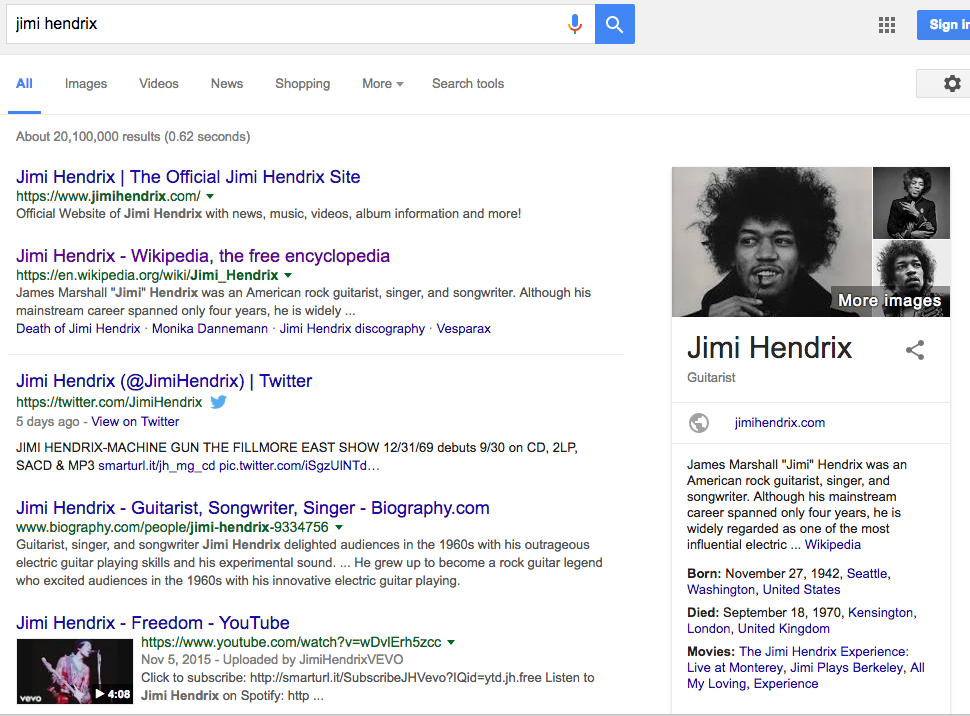
\includegraphics[width=0.8\textwidth]{./images/google_knowledge_graph}
  \caption[An example of knowledge graph application.]{An example of knowledge graph application in the Google's result page.}
  \label{fig:google_knowledge_graph}
\end{figure}

The use of Knowledge Graphs then allow users to be able to see extra information in a summarised table-like form, as to resolve their query without having to navigate to other sites. Note in the example in Figure \ref{fig:google_knowledge_graph} how the right column represents a sequence of facts of the \emph{\enquote{Jimi Hendrix}} entity, in this case an entity of the class (or type) \emph{PERSON}, such as: his official website; where and when he was born; where and when he died; and a list of movies where this person is the subject of.

Modern pipelines for building Knowledge Graphs from raw text would then encompass several Information Extraction techniques, such as the ones below:
\begin{enumerate}
  \item Discover entities in the text;
  \item Discover relationships between these entities;
  \item Perform entity disambiguation;
  \item Link entities to a reference Knowledge Graph (e.g., Yago2 \cite{Suchanek2007} or DBPedia \cite{dbpedia-swj});
  \item Improve the quality of the output via input data cleaning, robust extraction, and learning-based post-processing methods;
  \item Reason about how accurate these facts are;
  \item Finally presenting the facts in a graph (the Knowledge Graph).
\end{enumerate}

Some of these techniques will be explained further as part of this document.

In this project, we focus on studying and presenting some Information Extraction techniques as to build a domain-specific verb-centric information extraction tool that extracts relations from academic papers. More specifically, we focus on papers from the topic of databases and attempt to extract information from these papers for posterior usage by other systems with applications such as:
\begin{itemize}
	\item Allow for structured and fast search of techniques in the papers and the possible relations between them;
	\item Possibly group papers by their used techniques;
	\item Discovery of techniques to improve performance on a certain problem;
	\item Generate a hierarchy of concepts, and their use;
	\item Among others.
\end{itemize}

An existing service that organises data from academic papers is the Semantic Scholar \cite{semanticscholar} project, by Professor Oren Etzioni from Allen Institute for AI. However, Semantic Scholar only understands a limited number of relationships (such as 'cite', 'comment', 'use\_data\_set', and 'has\_caption') which are also more closely related to the meta-data about the paper, but not from the knowledge that the paper itself presents. Other similar services are Microsoft Academic Graph \cite{microsoft-academic-data}, Google Scholar \cite{google-scholar}, and CiteSeerX \cite{citeseer-x}.

In the next sections, this document will give some background information on the techniques needed to achieve the above (Chapter \ref{chapter:information}), and it will also define the problem more precisely (Chapter \ref{chapter:analysis}), building as to introduce the development of this research (Chapter \ref{chapter:developed}). In Chapter \ref{chapter:results} we will describe some of the results, followed by the some final remarks in Chapter \ref{chapter:conclusion}.


%
%
% INFORMATION EXTRACTION
%
%


\chapter{Information Extraction}
\label{chapter:information}
\pdfbookmark{Information Extraction}{pdfmark:infor}

Information Extraction, a term already defined in the introduction, is a hard problem which mostly relies in attempting to use a computer to understand information explicitly stated in the form of natural language.

It is interesting to observe that, before writing down thoughts in a paper, an academic form the ideas of what facts he/she wants to express in his/hers head, and then attempt a structure to most clearly state these in text form. These multiple facts, and the relations between them, are then stated in a sentence in what is assumed to be a somewhat logical format, following the semantics of the language, whether English or any other. Following this example, one must then also assume that the future reader of this paper will use the reverse process to decode this information into facts or ideas to be understood. In fact, this assumption is what justifies the attempt of Information Extraction.

Several initiatives in the Natural Language Processing area attempt to understand and map what these semantic rules are, and how one could use a computer for tackling natural language related tasks. These initiatives are fruitful and provide advanced tools and techniques in which some will be described in this chapter.


%
%
% NATURAL LANGUAGE PROCESSING
%
%


\section{Natural Language Processing}
\label{section:nlp}
\pdfbookmark{Natural Language Processing}{pdfmark:nlp}

\emph{Natural Language Processing} (or \emph{NLP}) can be a term used to discuss any kind of computer manipulation of natural language text, also called raw text. It can mean simple things such as counting words and obtain their frequency distribution to compare different writing styles, or in a more complex sense it would require the understanding of human writings, to the extent of being able to extract information and meaning from it, or also give useful responses to them \cite{BirdKleinLoper09}. On this more complex end of the spectrum, where one wants to understand raw text, language technology and existing tools rely on formal models, or representations, of knowledge of language at the levels of morphology, syntax, semantics, among others linguistic concepts. A number of formal models including state machines, formal rule systems, logic, and probabilistic models are used to capture this knowledge from text and reason with it \cite{Jurafsky:2000:SLP:555733}.

When information is laid out in natural language form, one start the analysis of the information presented by constructing a phrase or sentence based on smaller pieces of information such as verbs, nouns, and adjectives which are called the constituents. These then build up to form sequences of simple and complex sentences.

Observing more carefully a simple sentence, such as \emph{\enquote{The police chased him.}}, it is possible to attempt to sample the different syntactic information presented in it As a first step it is possible to dissect its constituent parts as per Figure \ref{fig:pos_tags}.

\begin{figure}[!htbp]
  \centering
    \texttt{The/DT police/NN chased/VBD him/PRP ./.}
  \caption[An example of tagged sentence.]{An example of tagged sentence.}
  \label{fig:pos_tags}
\end{figure}

The first word in the sentence, \emph{The}, is a \emph{DT} or determiner. Other possible determiners include \emph{\enquote{my}}, \emph{\enquote{your}}, \emph{\enquote{his}}, \emph{\enquote{her}}. The second word is \emph{\enquote{police}} is a \emph{NN} which is the tag for a singular noun. With this information we can already tell that this sentence is speaking about something, and this something is the noun \emph{\enquote{police}}. Subsequently the tag \emph{VBD} is presented which specifically indicates the word \emph{\enquote{chased}} is a verb (an action) in the past tense. At this point one can observe that something or someone (in this case the \emph{\enquote{police}}) did something in the past.

This is already great information to have about the sentence. These tags that were added to the text in Figure \ref{fig:pos_tags} are called Part-Of-Speech tags, or POS tags \cite{Jurafsky:2000:SLP:555733}. The standardization of these tags and work to develop and tag existing text with them is done by the Penn Treebank project \cite{Marcus:1993:BLA:972470.972475}.

\begin{table}[!htbp]
  \centering
    \begin{tabular}{lll}
      \textbf{POS tag}     & \textbf{Meaning}      & \textbf{Sample} \\
      ADP  & Adpositions                           & \emph{at}, or \emph{in}        \\  
      CONJ & Coordinating conjunction              & \emph{and}, or \emph{or} \\
      DT   & Determiner                            & The                     \\
      JJ   & Adjective                             & She is \emph{tired}     \\
      JJR  & Adjective, comparative                & That one is \emph{larger} \\
      JJS  & Adjective, superlative                & That is the \emph{largest}     \\
      NN   & Noun, singular or mass                & Car                     \\
      NNS  & Noun, plural                          & Cars                    \\
      NNP  & Proper noun, singular                 & Microsoft               \\
      NNPS & Proper noun, plural                   & The \emph{Kennedys}            \\
      RB   & Adverb                                & She said \emph{firmly}         \\
      VB   & Verb, base form                       & Attack                  \\
      VBD  & Verb, past tense                      & Attacked                \\
      VBG  & Verb, gerund or present participle    & Attacking               \\
      VBN  & Verb, past participle                 & Broken                  \\
      VBP  & Verb, non-3rd person singular present & I \emph{attack}                \\
      VBZ  & Verb, 3rd person singular present     & He \emph{attacks}               
    \end{tabular}
  \caption[List of some of the possible Part-Of-Speech (POS) tags.]{List of some of the possible Part-Of-Speech (POS) tags.}
  \label{tab:pos_tags_list}
\end{table}

Note how specific the tags are, dictating the type of the word, a verb for an example, and its variation either in quantity or tense. Some other examples of these tags are shown in Table \ref{tab:pos_tags_list}. Although most of them are simple to understand, note that \emph{ADP} are the adpositions, which encompasses prepositions and postpositions. Some systems, such as the spaCy Natural Language Processing parser \cite{honnibal-johnson:2015:EMNLP, spacy} also maps these more specific tags into more general ones, for an example, while three different words in a sentence are tagged independently as \emph{VBD}, \emph{VBG} and \emph{VBZ}, they are also tagged with a \emph{VERB} tag. This is useful, if the user is not too interested in the detail of which verb variation was used.

A Part-Of-Speech Tagger is then a system that, given a raw text as input, assigns parts of speech to each word (or token) and is able to produce as output the tagged version of this text. The text in Figure \ref{fig:pos_tags} was tagged using the Stanford Log-linear Part-Of-Speech Tagger \cite{Toutanova:2003:FPT:1073445.1073478}.

\begin{table}[!htbp]
  \centering
    \begin{tabular}{llll}
      \textbf{POS Tag} & \textbf{Word} & \textbf{Prev. Word} & \textbf{Prev. Tag}  \\
      DT               & The           & <START>             & <START>             \\
      NN               & police        & The                 & DT                  \\
      VBD              & chased        & police              & NN                  \\
      PRP              & him           & chased              & VBD                 \\
      .                & .             & him                 & PRP                 \\             
    \end{tabular}
  \caption[Features for sequential POS tagging.]{Features for sequential POS tagging.}
  \label{tab:pos_tags_features}
\end{table}

The task of assigning these tags starts by deciding what are the tokens in a raw text sentence, and what are its sentences. As an example, the tokenizer needs to decide if a period symbol near a word represents an abbreviation (e.g. \emph{Dr.}) or a sentence boundary - in case of an abbreviation, this period is then considered simply a token within the sentence. Another common problem in this step is deciding if a single quote is part of a word,(e.g. \emph{\enquote{It's}}), or is delimiting a quoted part of the sentence, thus potentially hinting other semantic meanings. The Stanford POS Tagger used in this example also contain a tokenizer, which is part of the Stanford CoreNLP \cite{manning-EtAl:2014:P14-5}, a set of natural language analysis tools.

Modern POS Taggers tackle this task using a technique called Sequence Classification. A machine learning classifier model is then trained with a corpus of manually tagged text and has as an input certain features that might indicate which tag a token being currently analysed should be assigned with. Observing again the example from Figure \ref{fig:pos_tags}, but now presented in table format in Table \ref{tab:pos_tags_features}, it is easier to see how this learning algorithm would be trained to predict tags on unseen test. Note the second word \emph{\enquote{police}}. For this word we are providing 4 features for the learning algorithm: the manually labelled POS Tag, the word itself, the previous word and the previous POS Tag. Suppose now that this sentence is included in a bigger corpus, and this pattern is a common one and the learning algorithm is provided with a substantial amount of labelled data in which this situation repeats itself: a \emph{NN} is the second word in a sentence, with \emph{\enquote{The}} and \emph{DT} being the previous word and tag respectively.

After the training, this model would behave in a similar fashion once presented with unseen data. Suppose now the first column on Table \ref{tab:pos_tags_features} is not presented. The model would pick the first word \emph{\enquote{The}} and observe the features: \emph{<START>} and \emph{<START>} respectively and given that in our previously described corpus this is a common occurrence, it would then label this word with \emph{DT}. Now, for the second word \emph{\enquote{police}}, the features would be \emph{\enquote{The}} for previous word, and \emph{DT} for previous tag. Again, it is common for a noun to be placed after a determiner so the model assigns the label \emph{NN} to the word \emph{\enquote{police}}. The features used by the Sequence Classifies both while training and when using the model may vary and they impact the quality of the predictions it makes. The Stanford POS Tagger uses a broad use of lexical features, including jointly conditioning on multiple consecutive words \cite{Toutanova:2003:FPT:1073445.1073478}.

A helpful concept at this stage is known as the lemma. A lemma is a canonical way of representing a word which strips out variations for quantity, tense, among others \cite{Jurafsky:2000:SLP:555733}. For an example, given the words \emph{\enquote{running}} or \emph{\enquote{runs}}, NLTK \cite{BirdKleinLoper09} outputs \emph{run} as their lemma. The lemma can, for an example, be used together or instead of the existing features for training models.

\begin{figure}[!htbp]
  \centering
    \texttt{Jetstar/NNP Airways/NNPS ,/PUNC a/DET unit/NN of/ADP Qantas/NNP Airways/NNP Limited/NNP}
  \caption[An example of another tagged sentence.]{An example of another tagged sentence.}
  \label{fig:pos_tags_2}
\end{figure}

When reading a text, it is also important to understand the relation between the words or sub-sentences that are contained in the phrase, and this is specially useful for information extraction. As an example, suppose the sentence \emph{\enquote{Jetstar Airways, a unit of Qantas Airways Limited}}. There are different ways of breaking down the relationship of the words in this sentence. 

Starting again with the POS tagging discussed earlier, one can see in Figure \ref{fig:pos_tags_2} what are the types of the words that constitutes this sentence. As a further step, it's possible to see what are the sub-sentences or parts that form the phrase structure, also called constituency parsing. The sub-sentences are connected upwards to one head (also called, \emph{parent}), and downwards to one or more governors (also called \emph{dependants}, or \emph{children}), in a recursive structure.  In Figure \ref{fig:sub_sentences_phrase_structure}, the phrase \emph{\enquote{of Qantas Airways Limited}}, which is part of the bigger phrase we are using as an example, is a prepositional phrase. A prepositional phrase lacks either a verb or a subject, and serve to assert binary relations between their heads and the constituents to which they are attached, in this case \emph{\enquote{a unit}} \cite{Jurafsky:2000:SLP:555733}. The sub-sentence \emph{\enquote{a unit of Qantas Airways Limited}} is then a noun phrase, since it contains and talks about a noun \emph{\enquote{unit}}.

\begin{figure}[!htbp]
  \centering
\Tree[.NP [.NP [.NNP \textit{Jetstar} ]
               [.NNPS \textit{Airways} ]]
          [.PUNC [., ]]
          [.NP [.NP [.DT \textit{a}    ]
                    [.NN \textit{unit} ]]
               [.PP [.IN \textit{of}    ]
                    [.NP [.NNP \textit{Qantas} ]
                         [.NNP \textit{Airways} ]
                         [.NNP \textit{Limited} ]]]]]
  \caption[A sentence and its components.]{A sentence broken down to its Phrase Structure (sub-sentences), also known as constituency parsing.}
  \label{fig:sub_sentences_phrase_structure}
\end{figure}

After discovering the structure between the phrases and its sub-phrases, finding the syntactical dependency between words themselves is also a very interesting and useful task. Continuing on the same example, one can see how the sentence states the simple fact that one company (\emph{Jetstar}) is a unit of another company (\emph{Qantas}). The Dependency Tree in this case tells us that \emph{Jetstar/NN} is the head of another noun \emph{Airways} and that the relation between them is of the \emph{compound} type. This relation is held between any noun that serves to modify the head noun and in this case indicate that this single entity is formed by two different words that are nouns. Note that \emph{Jetstar} has no parents and thus is the root of the sentence. The dependencies can be fully viewed is Figure \ref{fig:sub_sentences_dependency}.

The next relation is the \emph{appos} from \emph{\enquote{Airways}} to \emph{\enquote{unit}}. The appositional modifier relation indicates that the noun  immediately to the right of the first noun that serves to define or modify the meaning of the former. One now already knows that \emph{\enquote{Jetstar Airways}} is a \emph{\enquote{unit}}, and, in the business context, it probably means that it is a company that belongs to a bigger company.

\begin{figure}[!htbp]
  \centering
\begin{dependency}[theme = simple]
   \begin{deptext}[column sep=1em]
      Jetstar \& Airways \& , \& a \& unit \& of \& Qantas \& Airways \& Limited \\
   \end{deptext}
   \deproot{1}{ROOT}
   \depedge{2}{1}{compound}
   \depedge{2}{5}{appos}
   \depedge{5}{4}{det}
   \depedge{5}{6}{prep}
   \depedge[edge start x offset=+2pt]{6}{9}{pobj}
   \depedge{9}{7}{compound}
   \depedge[arc angle=50]{9}{8}{compound}
\end{dependency}
  \caption[A sentence and the dependencies between the words.]{A sentence and the dependencies between the words.}
  \label{fig:sub_sentences_dependency}
\end{figure}

Continuing the analysis, the next relation is of the \emph{prep} type and it indicates a prepositional modifier of a verb, adjective, or noun (our case), and it serves to modify the meaning of the verb, adjective, noun, or even another preposition. Note that this relation simply indicates the word pointed to by the edge is the preposition (in this case \emph{\enquote{of}}). The next relation, \emph{pobj}, indicates the actual object of the preposition and the noun phrase following the preposition and what it related to. This tree was created by the spaCy dependency parser \cite{honnibal-johnson:2015:EMNLP, spacy}. This same tree can be visualised in a more traditional tree structure in Figure \ref{fig:sub_sentences_dependency_tree}. Although not in this example, another very common relation is the relative clause modifier \emph{recmod} (or \emph{relcl} in some notations) relation. A relative clause modifier of an NP (\emph{Noun Phrase}) is a relative clause modifying the NP. The relation then in the tree points from the head noun of the NP to the head of the relative clause, normally a verb. The explanations for the cited relations in this document were obtained from the Stanford typed dependencies manual \cite{Marneffe08stanfordtyped}, and the Universal Dependencies (UD) project \cite{universal-dependencies-11234/1-1699}, both which are reference for the possible relation and contain a full lists of their meanings.

\begin{figure}[!htbp]

\centering
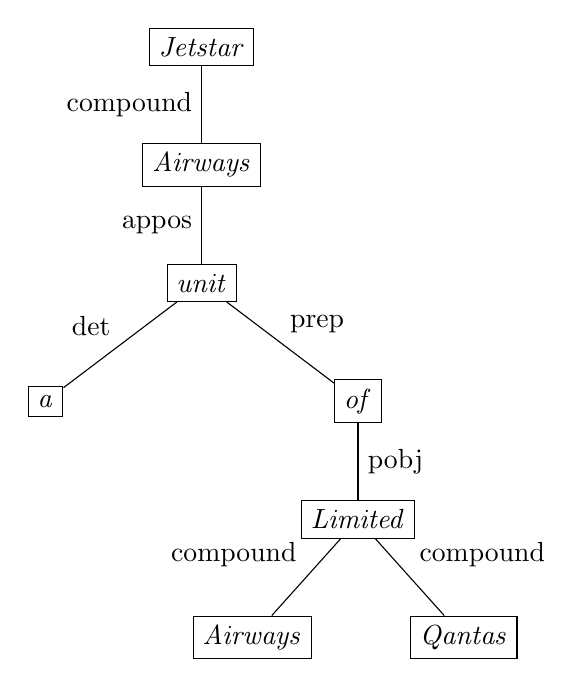
\begin{tikzpicture}[every tree node/.style={draw},
   level distance=1.50cm,sibling distance=1.25cm,
   edge from parent path={(\tikzparentnode) -- (\tikzchildnode)}]
\Tree
[.\textit{Jetstar} \edge node[auto=right] {compound};
		[.\textit{Airways} \edge node[auto=right] {appos};
			[.\textit{unit} 
				 \edge node[auto=right] {det}; [.\textit{a} ]
				  \edge node[auto=left] {prep}; [.\textit{of}
				  	\edge node[auto=left] {pobj}; [.\textit{Limited}
				  		\edge node[auto=right] {compound}; [.\textit{Airways} ]
				  		\edge node[auto=left] {compound}; [.\textit{Qantas} ] ] ] ] ] ] 
\end{tikzpicture}

\caption[A sentence and the dependency tree, showing the syntactical relation between these words.]{A sentence and the dependency tree, showing the syntactical relation between these words.}
\label{fig:sub_sentences_dependency_tree}
\end{figure}

The software that is able to output a syntactical dependency tree, given a sentence, is called a dependency parser. Several different methods can be used to achieve this. One way is by defining dependency grammars, and then parsing text using these grammars. The grammar would contain words and its possible heads, and it would be applied repeatedly into the text in a process called cascaded chunking \cite{BirdKleinLoper09}. More recent methods use a process called Shift-reduce, in which the sentence is kept in a queue with the left-most token in front of the queue. The model could then decide between applying 3 operations:
\begin{enumerate}
  \item Shift: move one token from the queue to stack.
  \item Reduce left: top word on stack is head of second word.
  \item Reduce right: second word on stack is head of top word.
\end{enumerate}

A model is then trained to predict, given a text that is added to the queue, what is the next move that it should take, and what is the sequence of moves that will result in the best possible final dependency tree. This is done in a monotonic manner, in the sense that once a decision is made by the model, it cannot change it. Full working examples of this method are described in \cite{chen-manning:2014:EMNLP2014}. Other methods also use these 3 possible decisions, but allow the parser to be non-monotonic and go back in the tree and change previous decisions given new evidence form the features, such as spaCy and its dependency parser \cite{honnibal-johnson:2015:EMNLP, spacy}. Another method also uses the same set of decisions, but does a beam-search observing multiple partial hypotheses and keeping them at each step, with hypotheses only being discarded when there are several other higher-ranked hypotheses under consideration, such as the Syntaxnet parser \cite{google-syntaxnet, DBLP:journals/corr/AndorAWSPGPC16}. All these cited models use neural networks as the method to form the model.

As a further example, besides providing dependency parsing tree, spaCy also provides an iterator so you can obtain what is called the noun chunks of the document. The noun chunks are smaller pieces of the sentences within the document that are base noun phrases, or a 'NP chunk' (as per Figure \ref{fig:sub_sentences_phrase_structure}). They are noun phrases that do not permit other NPs to be nested within it – so no NP-level coordination (e.g.: \emph{\enquote{cat/NN and/CONJ dog/NN}}), no prepositional phrases, and no relative clauses \cite{spacy}.

Other problems tackled by the Natural Language Processing discipline and that are relevant for Information Extraction are \emph{Coreference resolution} and \emph{pronominal anaphora resolution}. Coreference resolution intends to define all possible entities that a text can reference to in some sort of definitive list, or more precisely a \emph{discourse model}, find in the text all the chained references to these entities, and link them to the specific entities. While very similar in nature, pronominal anaphora resolution is more simple as it is the problem of resolving in a given sentence to which previous NN (noun) or NNP (proper noun) a single PRP (pronoun) refers to \cite{Jurafsky:2000:SLP:555733}.

Take for an example the sentence \emph{\enquote{John is a quiet guy, but today he is furious.}}, the initial mention of the entity \emph{John} appears in the first token. Token five talks about a \emph{guy}, which although not a pronoun, is still a reference to the previous entity in the first word. The ninth token is a pronoun and again refers to the same \emph{John}, so is part of the chain of mentions. The full resolution chain would be denoted in Figure \ref{fig:sub_sentences_coreference}.

Normally these systems work towards analysing pairs of tokens using a probabilistic model, and then decide how likely they are references for the same entity. More recent approaches also group possible tokens in a cluster and use cluster-level features to determine the chains of coreferences \cite{clark2015entity}. The tool used to extract Figure \ref{fig:sub_sentences_coreference} is the Stanford Coreference Resolution annotator \cite{clark2015entity}, which is part of the latter group of tools that use cluster level features. This annotator is also part of the CoreNLP toolset \cite{manning-EtAl:2014:P14-5}.

\begin{figure}[!htbp]
  \centering
\begin{dependency}[theme = simple]
   \begin{deptext}[column sep=1em]
      John \& is \& a \& quiet \& guy \& , \& but \& today \& he \& is \& furious \& . \\
   \end{deptext}
   \deproot{1}{mention}
   \depedge{9}{5}{coref}
   \depedge{5}{1}{coref}
\end{dependency}
  \caption[A sentence, the mentions of an entity, and the proposed coreference resolutions.]{A sentence, the mentions of an entity, and the proposed coreference resolutions.}
  \label{fig:sub_sentences_coreference}
\end{figure}

All linguistic data mentioned in this section is data that can be obtained from the raw text itself, and is then the base for several features in which methods for Information Extraction act on.


%
%
% INFORMATION EXTRACTION
%
%


\section{Information Extraction}
\label{section:information_extraction}
\pdfbookmark{Information Extraction}{pdfmark:ie}

The IE (Information Extraction) process is described by the following subtasks: Named Entity Recognition (NER), Coreference Resolution, Entity Disambiguation, Relation Extraction (RE), Event Detection, and Temporal Analysis \cite{Jurafsky:2000:SLP:555733}. The main subtasks relevant to this report will be described further in this section.

Once the information is extracted it is then used for tasks such as Template Filling \cite{Jurafsky:2000:SLP:555733}, Question and Answering systems \cite{Moens:2006:IEA:1177314}, or stored as a Knowledge Graph for downstream logical reasoning or for further queries.

\begin{table}[!htbp]
  \centering
  \RaggedRight
    [\textsubscript{PER} James Cook] was born on 27 October 1728 in the village of [\textsubscript{LOC} Marton] in [\textsubscript{COUNTY} Yorkshire].
  \caption[An example of NER.]{An example of Named Entity Recognition (NER).}
  \label{tab:james_cook}
\end{table}

Named Entity Recognition (NER) is the process of, given a sentence, identify and extract what are the entities that are part of it. Once the entity is detected, it needs to be classified within the classes of the given domain - in the spirit of the previous examples this would be e.g.: \emph{CITY} or \emph{PERSON}. Different types of entities are relevant to context of the data being worked with. A few approaches exist for the problem of NER, mostly related to Pattern Matching or Sequence Classification.

\begin{table}[!htbp]
  \centering
    \begin{tabular}{ll}
      \textbf{Pattern}          & \textbf{Would yield ENTITY of type} \\
      {[PERSON]} was born       & PERSON            \\
      in the village of {[LOC]} & LOCATION          \\
      in {[LOC]}                & LOCATION           
    \end{tabular}
  \caption[Patterns for NER.]{Examples of Named Entity Recognition (NER) patterns, based on the sentence from Table \ref{tab:james_cook}.}
  \label{tab:james_cook_patterns}
\end{table}

Observe, for an example, the sentence in Table \ref{tab:james_cook}. Several articles regarding prominent figures, either historical or of our current society, can be of the format \emph{\enquote{Jimi Hendrix was born}}. One approach might be Pattern Matching, which is to mine the input natural language text while looking for the pattern \emph{\enquote{[ENTITY] was born}}, using Regular Expressions (Finite-State Automata) \cite{Jurafsky:2000:SLP:555733}. The entities found by this pattern would then also receive the \emph{PERSON} class. This pattern would miss the sentence \emph{\enquote{Jimi Hendrix, born in Seattle}} since it does not fit the pattern and, because of this, one generally needs to build a list or database of patterns to work with in a corpus. An example of such database was generated by the PATTY system \cite{Nakashole:2012:PTR:2390948.2391076}. Table \ref{tab:james_cook_patterns} depicts other possible similar patterns.

Another way to extract entities from text is to frame the NER problem as a Sequence Classification problem, similar to the POS tagging problem described earlier. It requires the training of a classifier in which, given the class of the previous word, and other surrounding features of the current word, will attempt to guess if the current word is an entity, and if it is, also guesses its class.

To achieve this, previously annotated data with existing sentences and its entities is needed. This can be obtained by manually labelling data, or by semi-automated methods, like the one proposed later by this document. The format in which this annotated data is provided varies, however the IOB format (Table \ref{tab:james_cook_iob}) is more commonly used in several of the NER tools, including NLTK \cite{BirdKleinLoper09} and the popular Stanford Named Entity Recognizer (NER) \cite{Finkel:2005:INI:1219840.1219885}, part of the Stanford CoreNLP \cite{manning-EtAl:2014:P14-5}. Stanford CoreNLP provides a set of natural language analysis and information extraction tools.

\begin{table}[!htbp]
  \centering
    \begin{tabular}{ll}
      \textbf{Word}          & \textbf{Tag} \\
      James                  & B-PERSON \\
      Cook                   & I-PERSON \\
      was                    & O \\
      born                   & O \\
      on                     & O \\
      27                     & B-DATE \\
      October                & I-DATE \\
      1728                   & I-DATE \\
      in                     & O \\
      the                    & O \\
      village                & O \\
      of                     & O \\
      Marton                 & B-LOC \\
      in                     & O \\
      Yorkshire              & B-LOC \\
      .                      & O \\
    \end{tabular}
  \caption[IOB-formatted sentence.]{Example of IOB-formatted sentence used to train classifiers for the Named Entity Recognition (NER) task, based on the sentence from Table \ref{tab:james_cook}.}
  \label{tab:james_cook_iob}
\end{table}

The IOB format also helps remove ambiguity in case there are two contiguous entities of same class without any word tagged as \emph{O} in between. In practice these cases are somewhat rare in several domains, and even when trained with such tags classifiers struggle to accurately determine the boundaries of an entities, and thus a simplified version of this annotation without the \emph{B-} and \emph{I-} prefixes is more commonly used \cite{Surdeanu:2011:CIE:2021153.2021155}.

The Stanford Named Entity Recognizer (NER), also known as CRFClassifier \cite{Finkel:2005:INI:1219840.1219885}, provides a general implementation of (arbitrary order) linear chain Conditional Random Field (CRF) sequence models. A CRF is a conditional sequence model which represents the probability of a hidden state sequence given some observations.

Several relevant features can be used as an input during the training of a NER CRF classifier model. In Table \ref{tab:ner_features}, examples are presented. The Word Shape feature is an interesting addition from recent research, as it captures the notion that most entities are written in capital letters, or starting with capital letter, or containing numbers in the middle of the word, and other specific shapes.

\begin{table}[!htbp]
  \centering
    \begin{tabular}{ll}
      \textbf{Feature}          & \textbf{Description} \\
      Word                      & The current word being classified.          \\
      N-grams                   & \parbox[t]{9cm}{A feature from n-grams, i.e., sub-strings of the word.} \\
      Previous Class            & The class of the immediate previous word.          \\
      Previous Word             & The previous word.          \\
      Disjunctive               & \parbox[t]{9cm}{Disjunctions of words anywhere in the left or right.} \\
      Word Shape                & \parbox[t]{9cm}{The shape of the word being processed captured using. In general replaces numbers with \emph{d}, \emph{x} to lower-case letters, and \emph{X} to upper-case letters.} \\
    \end{tabular}
  \caption[Possible features to train the CRFClassifier.]{Examples of features used to train the CRFClassifier \cite{Finkel:2005:INI:1219840.1219885}.}
  \label{tab:ner_features}
\end{table}

In addition to the above methods another useful technique is the use of gazetteers. Gazetteers are common for geographical data, where government provided lists of names can contain millions of entries names for all manner of locations along with detailed geographical, geologic and political information \cite{Jurafsky:2000:SLP:555733}.

Relation Extraction (RE) is the ability to discern the relationships that exist among the entities detected in a text \cite{Jurafsky:2000:SLP:555733}, and is naturally the next challenge after being able to detect entities. It is generally denoted as a triplet: two entities, and the one relation between them (Table \ref{tab:relation_example}). It can be done using Pattern Matching, Classifiers, or purely by exploiting linguistic data available form a sentence. The previously described Pattern Matching technique from NER can be improved upon in the Relation Extraction step, and involve more than one entity, yielding binary relations. This approach is used in tools such as PROSPERA \cite{Nakashole:2011:SKH:1935826.1935869} or those mined by PATTY \cite{Nakashole:2012:PTR:2390948.2391076}. More specifically, examples of patterns mined by PATTY for the \emph{graduatedFrom} relation are seen in Figure \ref{fig:patty_examples}.

\begin{table}[!htbp]
  \centering
  \RaggedRight
    \texttt{Located\_In(Kiel, Germany)} \\
  \caption[An example of a triplet that represents a relation.]{An example of a triplet that represents a relation.}
  \label{tab:relation_example}
\end{table}

\begin{figure}[!htbp]
  \centering
    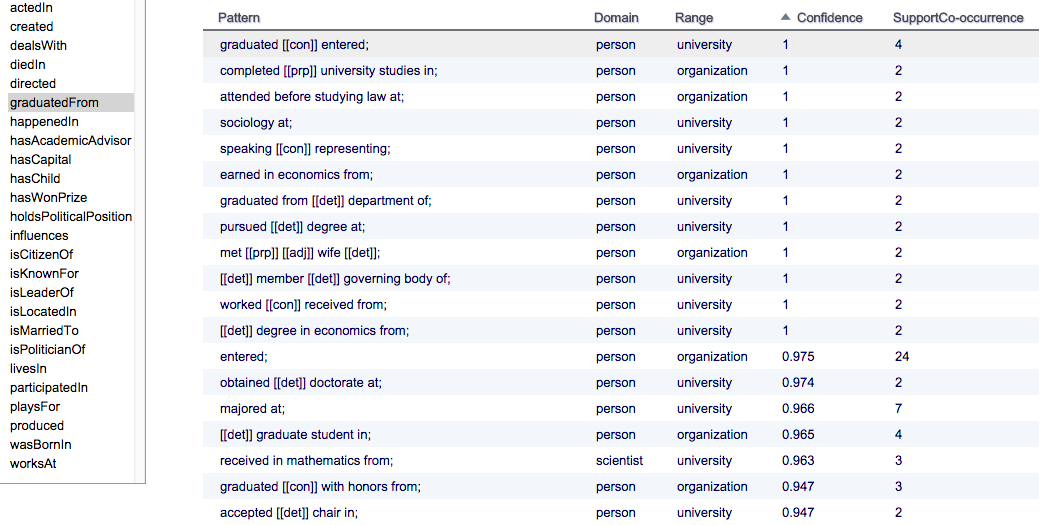
\includegraphics[width=0.8\textwidth]{./images/patty}
  \caption[An example of patterns extracted from PATTY.]{An example of patterns extracted from PATTY for the \emph{graduatedFrom} relation.}
  \label{fig:patty_examples}
\end{figure}

PROSPERA's main technique is that not only it obtain facts based on a small set of initial seed patterns, but also obtain new candidate patterns that can be extrapolated from the corpus based on the mined known facts. Once the process of obtaining new candidate patterns finishes, these are evaluated and then added to the the existing pattern repository for re-use. The whole process then iterates again finding even more facts from these new patterns, and new candidate patterns \cite{Nakashole:2011:SKH:1935826.1935869}. Moreover, another interesting characteristic of the PROSPERA's approach is the care in Entity Disambiguation. For an example, given that in a text it finds a name, such as \emph{\enquote{Captain James Cook}}. It then uses a knowledge base such as YAGO \cite{Suchanek2007} to compare this with existing known entities, using techniques such as N-gram comparison \cite{Nakashole:2011:SKH:1935826.1935869}. With such effort, PROSPERA is able to know that \emph{Captain James Cook} and \emph{James Cook} are actually the same entity with a certain confidence, and thus don't differentiate these and assigns \emph{\enquote{Captain James Cook}} as a representation of the canonical unambiguous entity \emph{\enquote{James Cook}}. This helps in several ways, such as: it can then know other information about this entity, such as the fact that it is of the class \emph{PERSON}; and it can also facilitate future queries in this knowledge base, centralizing the new information found about this existing entity.

Another tool in the Stanford CoreNLP package, the Relation Extractor \cite{Surdeanu:2011:CIE:2021153.2021155} is a classifier to predict relations in sentences. This program has a model that extracts binary relations between entity mentions in the same sentence. The output is normally in the XML \cite{xml} format and denotes the tokens of each sentence, the possible relations, and the confidence level of these relations. The XML demonstrated in Figure \ref{fig:xml_output1} depicts a guess that 2 words in the sentence \emph{\enquote{..., including approaches that use parallel computation [1, 2, 6, 13, 24].}} have the \emph{Uses} relation with a confidence above 70\%. The classifier in this case also indicates that one of the entities is of the class \emph{CONCEPT}.

\begin{figure}[!htbp]
  \centering
    \lstset{
    language=xml,
    tabsize=3,
    %frame=lines,
    %caption=Test,
    %label=code:sample,
    %frame=shadowbox,
    rulesepcolor=\color{blue},
    xleftmargin=20pt,
    framexleftmargin=15pt,
    keywordstyle=\color{blue}\bf,
    commentstyle=\color{OliveGreen},
    stringstyle=\color{red},
    numbers=left,
    numberstyle=\tiny,
    numbersep=5pt,
    breaklines=true,
    showstringspaces=false,
    basicstyle=\footnotesize,
    emph={relation,arguments,entity,span,probabilities,probability,label,value},emphstyle={\color{blue}}
    }
    \lstinputlisting{images/relations.xml}
  \caption[An example of relation extracted with the Stanford Relation Extractor.]{An example of relation extracted with the Stanford Relation Extractor that demonstrated the \emph{\enquote{Uses}} relation.}
  \label{fig:xml_output1}
\end{figure}

As part of its training, annotated relation mentions are used as an input together with the text it belongs to, and the annotation becomes a positive example for the corresponding label, while all the other possible combinations between entity mentions in the same sentence become negative examples. The feature set models the relation between the arguments by using the distance between the relation arguments, the syntactic path between the two arguments, using both constituency and dependency representations.

Note how at this point it's important to note the notion of a \emph{pipeline} of natural language processing tasks. Stanford's CoreNLP is able to, by itself, perform all the steps needed to produce such relation extraction output from the raw text input. The steps of this pipeline are executed in a certain order, as they depend on the previous step (e.g.: POS tagging is needed for Dependency Parsing). In this case, the process was:

\begin{enumerate}
  \item Tokenize;
  \item Sentence Splitter;
  \item Part-of-Speech tagging;
  \item Lemmatization;
  \item Constituency parsing;
  \item Dependency Parsing;
  \item Named Entity Recognition;
  \item and finally, Relation Extraction.
\end{enumerate}

The Stanford Relation Extractor comes with a model that was trained to extract the following relations: \emph{Live\_In}, \emph{Located\_In}, \emph{OrgBased\_In}, \emph{Work\_For} - and the following classes: \emph{PERSON}, \emph{ORGANIZATION}, \emph{LOCATION}. There are big challenges if one attempts to train the model for any relation outside of these, mainly in obtaining or generating annotated data to train the classifier as to generate a useful model. There are attempts in which relation extraction is not based on annotated data, but on linguistic characteristics of the text itself, such as its semantics. These tools are normally called Open Relation Extractors and will be further described in Section \ref{section:related}.


%
%
% KNOWLEDGE GRAPHS
%
%


\section{Knowledge Graphs}
\pdfbookmark{Knowledge Graphs}{pdfmark:kg}


Knowledge Graphs contain a valuable of information in a structured format, traditionally originally mined from table-like structures form places like Wikipedia \cite{wiki} tables \cite{dbpedia-swj}, or from processes like Information Extraction as described in the previous section. It can be used for a diverse range of applications, such as helping other systems reason about quality of harvested facts \cite{Suchanek2007}, provide table-like facts about an entity \cite{google}, and question-answering systems \cite{hixon-clark-hajishirzi-2015}. Moreover, recent years have witnessed a surge in large scale knowledge graphs, such as DBpedia \cite{dbpedia-swj}, Freebase \cite{Bollacker2008}, Google’s Knowledge Graph \cite{google}, and YAGO \cite{Suchanek2007}.

\begin{figure}[!htbp]
  \centering
    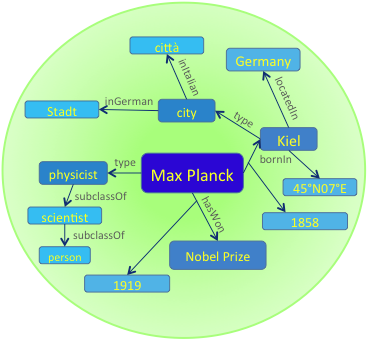
\includegraphics[width=0.6\textwidth]{./images/yago_graph}
  \caption[An example of knowledge graph plotted with vertices and edges.]{An example of knowledge graph from \cite{Suchanek2007} plotted with vertices and edges.}
  \label{fig:yago_knowledge_graph}
\end{figure}

The Knowledge Graph name follows from the data structure that is created from the facts in its final form, a graph with nodes representing entities and edges representing various relations between entities. In Figure \ref{fig:yago_knowledge_graph}, it is possible to observe an example plotted in this form. The list of possible entities classes, and allowable relations between entities is known as a schema. The schema represented in Figure \ref{fig:yago_knowledge_graph} is detailed in Table \ref{tab:max_planck}; one can observe that, as an example, \emph{\enquote{Max Planck}} is an entity of the type \emph{physicist}.

\begin{table}[!htbp]
  \centering
  \RaggedRight
    \texttt{type(A, D) :- type(A, B), subclassOf(B, C), subclassOf(C, D)} \\
  \caption[An example of entailment.]{This entailment example allows one to assert that \texttt{type(Max Planck, person)} is also true, based on the fact tuples presented in Table \ref{tab:max_planck}.}
  \label{tab:entailment_example_max}
\end{table}

\begin{figure}[!htbp]
  \centering
    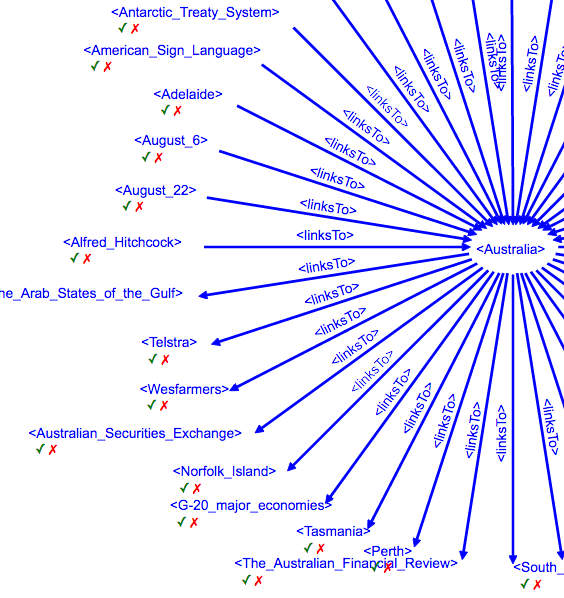
\includegraphics[width=0.6\textwidth]{./images/yago}
  \caption[An example of patterns existants in YAGO.]{An example of patterns existants in YAGO.}
  \label{fig:yago_examples}
\end{figure}

Moreover, based on the facts presented, entailments can be made and one trivial example is denoted in Table \ref{tab:entailment_example_max}. More complex examples of possible reasoning can be seen in \cite{Surdeanu:2011:CIE:2021153.2021155}. This is equivalent to traversing the graph from a node that represents a more specific information, to a node that represents a more general information - e.g.: another possible child node of \emph{\enquote{scientist}} could be the type \emph{\enquote{biologist}}.

\begin{table}[!htbp]
  \centering
  \RaggedRight
    \texttt{type(Max Planck, physicist)} \\
    \texttt{subclassOf(physicist, scientist)} \\
    \texttt{subclassOf(scientist, person)} \\
    \texttt{bornIn(Max Planck, Kiel, 1858)} \\
    \texttt{type(Kiel, city)} \\
    \texttt{locatedIn(Kiel, Germany)} \\
    \texttt{hasWon(Max Planck, Nobel Prize, 1919)} \\
  \caption[Some facts regarding Max Planck.]{Some facts regarding Max Planck, also depicted in Figure \ref{fig:yago_knowledge_graph}.}
  \label{tab:max_planck}
\end{table}

This example denotes a classical domain, more precisely important persons, companies, locations, and the relations between them, in which Information Extraction (IE) tools have been very successful on.

As mentioned previously, YAGO \cite{Suchanek2007} is a prominent Knowledge Graph database, and possesses several advanced characteristics. Every relation in its database is annotated with its confidence value. See the example of the resulting graph in Figure \ref{fig:yago_examples}. Moreover, YAGO combines the provided taxonomy with WordNet \cite{Miller:1995:WLD:219717.219748} and with the Wikipedia category system \cite{wiki}, assigning the entities to more than 350,000 classes. This allow for very powerful querying. Finally, it attaches a temporal and a spacial dimension to many of its facts and entities, being then capable to answer questions such as \emph{when} and \emph{where} such event took place.

WordNet is a semantically-oriented dictionary of English, similar to a traditional thesaurus but with a richer structure \cite{BirdKleinLoper09}. More specifically, it provides relations to synonyms, hypernyms and hyponyms, among others.


%
%
% CHALLENGES AND RELATED WORK
%
%


\chapter{Analysis and Related Work}
\label{chapter:analysis}
\pdfbookmark{Analysis and Related Work}{pdfmark:related}

This work intends to deliver a tool or a process in which one can extract information from academic text, more specifically Computer Science papers form the Database and Data Mining topics. The intention is to obtain entities, and relations between these entities. The motivation is that, with such tool, one could for an example:
\begin{itemize}
	\item Historically research algorithms that were mostly used during a certain time period;
	\item Find which algorithms are used to resolve, or related to, a certain problem;
	\item Find techniques that improve a certain algorithm problem, among others.
\end{itemize}

\section{Analysis of Academic Text}
\label{section:analysis_of_academic_text}
\pdfbookmark{Analysis of Academic Text}{pdfmark:academic}

The corpus of text used was generated utilising papers published from the following conferences during various years: ACL \cite{acl}, EMNLP \cite{emnlp}, ICDE \cite{icde}, SIGMOD \cite{sigmod}, VLDB \cite{vldb}. More specifically, the section of \emph{Related Work of} these papers were the ones used to build the corpus. This was done due to the characteristics and patterns of this section compared to the rest of the paper. After careful reading, we observed that the \emph{Related Work} section generally contains objective comparisons between other algorithms or softwares in contrast with more opaque or abstract explanations form other parts of the paper. This would mean that this section was a good candidate to start the analysis from. Note the following examples of sentences from the \emph{Related Work} section of papers from the corpus:
\begin{enumerate}
	\item \emph{\enquote{Bergsma et al (2013) show that large-scale clustering of user names improves gender, ethnicity and location classification on Twitter.}}
	\item \emph{\enquote{N-Best ROVER (Stolcke et al, 2000) improves the original method by combining multiple alternatives from each combined system.}}
	\item \emph{\enquote{By partitioning the velocity space, the Bdual -tree improves the query performance of the B x -tree.}}
\end{enumerate}

Entities from academic text in this setting are not as straightforward to define as in, for an example, business news, or criminal news. Observe the following sentence:
\begin{itemize}
	\item \emph{\enquote{Japan's Toshiba Corp said it had nominated Satoshi Tsunakawa, a former head of its medical equipment division, to be its next chief executive officer.}}
\end{itemize}

\begin{table}[!htbp]
  \centering
    \begin{tabular}{ll}
      \textbf{Text}             & \textbf{Entity Type} \\
      Japan                     & LOCATION            \\
      Toshiba Corp              & ORGANIZATION          \\
      Satoshi Tsunakawa         & PERSON           
    \end{tabular}
  \caption[NER from the business news example.]{Examples of Named Entity Recognition (NER) from the business news text example.}
  \label{tab:entities_from_business_text}
\end{table}

From the news text example above, Table \ref{tab:entities_from_business_text} lists the entities that are clearly noted in the text. One can observe a very strong feature which is the common capitalization of the first letter of each of these entities. Another characteristic is how entities from this news text example are \emph{global} or \emph{unconditional}: \emph{\enquote{Japan}} is a location regardless of any condition or any context in this document. Another observation is that, referring to the Stanford's Relation Extraction default relations, \emph{\enquote{Toshiba Corp}} is an organisation \emph{Located\_In} \emph{\enquote{Japan}} regardless of other context in this document. This contrasts with concepts and their relations observed in academic papers, thus that while \emph{\enquote{large-scale clustering}} has the \emph{Improves} relation with \emph{\enquote{gender classification}} in the context of the paper where this data is presented, it might not be true in all cases.

\begin{table}[!htbp]
  \centering
    \begin{tabular}{ll}
      \textbf{Text}             & \textbf{Entity Type} \\
      Bergsma et al (2013)      & AUTHOR          \\
      large-scale clustering    & CONCEPT         \\
      gender classification     & CONCEPT         \\
      ethnicity classification  & CONCEPT         \\
      location classification   & CONCEPT         \\
      Twitter                   & ORG             \\
    \end{tabular}
  \caption[NER from the academic text example.]{Examples of Named Entity Recognition (NER) from the academic text example.}
  \label{tab:entities_from_academic_text}
\end{table}

Moreover, the entities in Table \ref{tab:entities_from_academic_text} are harder to classify in universally agreed classes. For an example, \emph{\enquote{gender classification}} can be considered an action, or a task, or an algorithm. More generally, one can simply classify these as concepts.

\begin{table}[!htbp]
  \centering
  \RaggedRight
    \texttt{IsA(Concept,Concept)} \\
    \texttt{SimilarTo(Concept,Concept)} \\
    \texttt{Improves(Concept,Concept)} \\
    \texttt{Employs(Concept,Concept)} \\
    \texttt{Uses(Concept,Concept)} \\
    \texttt{Supports(Concept,Concept)} \\
    \texttt{Proposes(Author,ComplexConcept)} \\
    \texttt{Introduces(Author,ComplexConcept)} \\
  \caption[Some observed and possible relations between concepts.]{Some observed and possible relations between concepts.}
  \label{tab:possible_academic_relations}
\end{table}

Other possible relations from the Stanford Relation Extractor standard relations that are applicable to the above news text example are: \emph{OrgBased\_In} (again for \emph{\enquote{Toshiba Corp}} and \emph{\enquote{Japan}}) and \emph{Work\_For} regarding its newly placed chief executive officer. Again, contrasting with the academic text, one might consider relations such as the one possibles between concepts as denoted in Table \ref{tab:possible_academic_relations}. In fact, by analysing the corpus for the top 50 words in the singular third-person form, such as \emph{\enquote{improves}} or \emph{\enquote{employs}}, one can have an idea of the possible relations that can be extracted. This process is illustrated in Figure \ref{fig:words_most_use_no_top2}: note that the top two words were removed from the graph (\emph{\enquote{is}} with a count of 41694, and \emph{\enquote{has}} with a count of 8157) as their usage counts are too high compared to the other words.

\begin{figure}[!htbp]
  \centering
    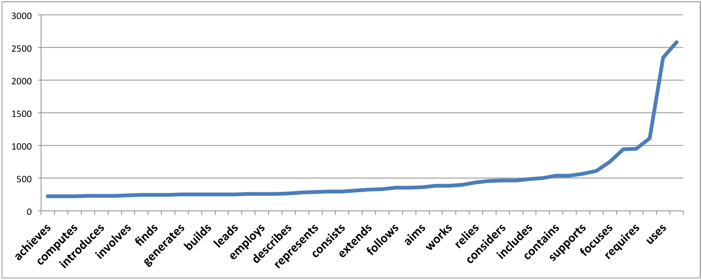
\includegraphics[width=1.0\textwidth]{./images/words_most_use_no_top2}
  \caption[Samples of the most common words in the singular third-person form, after removing the top 2 words.]{Samples of the most common words in the singular third-person form, after removing the top 2 words (\emph{\enquote{is}} and \emph{\enquote{has}}). The \emph{y} axis represents the number of times the word in the \emph{x} axis appeared in the text.}
  \label{fig:words_most_use_no_top2}
\end{figure}

One of the initial attempts to explore how to extract information from the generated corpus was to use the Stanford Named Entity Recognizer (NER) to recognize the concepts discussed so far in the academic text. To do so, a small set of around 20 papers' \emph{Related Work} section was annotated for the concepts contained in them using Brat \cite{Stenetorp:2012:BWT:2380921.2380942}. An example of this annotated data can be seen in Figure \ref{fig:brat_img}.

The annotated data is then transformed form Brat's standoff format \cite{Stenetorp:2012:BWT:2380921.2380942} into a Table Separated Value (TSV) format, using a custom script, based on customised version of from standoff2conll\footnote{\url{https://github.com/spyysalo/standoff2conll}}, renamed standoff2others. The output is similar to the one showed in Table \ref{tab:james_cook_iob}, but its simplified version without the \emph{B-} and \emph{I-} prefixes.

The model was trained mostly with the recommended settings and features, such as the word itself, its class, surrounding words and word shapes. When applying this trained NER model (Figure \ref{fig:stanford_ner_usage}), we observed that the success was moderated, as it was, at times, able to detect clearly delineated concepts by its shape (.e.g: capital words), but for non-capitalized words it appeared as it would only recognize the concepts if its words were present in the training set.

\begin{figure}[!htbp]
  \centering
    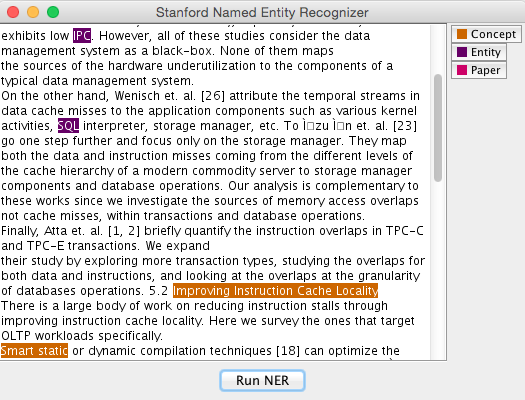
\includegraphics[width=0.9\textwidth]{./images/stanford_ner}
  \caption[The Stanford NER GUI (Graphic User Interface) using our trained model.]{The Stanford NER GUI (Graphic User Interface) using our trained model.}
  \label{fig:stanford_ner_usage}
\end{figure}

In this image, please observer the attempt of differentiate entities such as \emph{CONCEPT} and \emph{ENTITY}. We also annotated references to other papers using the \emph{PAPER} entity, in general they appears as numbers between square brackets. Initially, we attempted to annotated using a hierarchy where entities were very specific proper nouns, while concepts had a more loose definition, and would likely be more general concepts. During the process, however, this type of annotation also proved to be difficult as it would require domain-specific knowledge of very deep database discussions in order to differentiate concepts by these two classes, and could still sometimes generate debates.

As an attempt of further improve the quality of the NER model, we made use of a gazetteer. As part of this research, the Microsoft Academic Graph \cite{microsoft-academic-data} was found to contain a very relevant list of \emph{keywords} and \emph{fields of study} available for download and academic use. Another custom script was developed to transform the data from the format provided by Microsoft into the input format accepted by Stanford's NER shown in Table \ref{tab:concept_list_from_gazetteer}. The Stanford NER utilises the gazetteer input in both ways: matching the concepts token by token in their entirety, or in a \enquote{sloppy} manner accepting a positive match even if only one of the tokens in the gazetteer entry had a match \cite{Finkel:2005:INI:1219840.1219885}. In both cases, however, the gazetteer is treated simply as another feature and does not guarantee that if the entries are found in the text they would be marked as an entity \cite{Finkel:2005:INI:1219840.1219885}. The gazetteer format has its first token denoting the type of the entry, all of the type \emph{CONCEPT} in this case, with the following words denoting the gazetteer entry itself, space separated. We did not observed improvement with this addition.

\begin{table}[!htbp]
  \centering
    \begin{tabular}{l}
CONCEPT SMOOTHSORT \\
CONCEPT CUSTOMISED APPLICATIONS FOR MOBILE NETWORKS \\
CONCEPT XML DOCUMENTS \\
CONCEPT JOSEPHUS PROBLEM \\
CONCEPT RECOGNIZABLE 
    \end{tabular}
  \caption[Format in which Stanford's NER supports a gazetteer input.]{Format in which Stanford's NER supports a gazetteer input.}
  \label{tab:concept_list_from_gazetteer}
\end{table}

The next step was to attempt to use the Stanford Relation Extractor (RE). The same small annotated sample by us in Brat would also contain the following relations: \emph{Improves}, \emph{Worsen}, \emph{IsA}, \emph{Uses}. The standoff2others custom library was then improved to be able to generate the more complex CoNLL format, accepted as an input for training of the Stanford's RE, denoted in Table \ref{tab:format_for_relation_extractor_input} \cite{Surdeanu:2011:CIE:2021153.2021155}. Also, the Java parser code from the Relation Extractor had to be changed in a few places to accept custom labels (classes) for NER.

\begin{table}[!htbp]
  \centering
    \begin{tabular}{lllllllll}
2 &	Concept &	0 &	O &	NNP/NNS &	LSH/functions &	O &	O &	O \\
2 &	O &	1 &	O &	VBP &	are & 	O &	O &	O \\
2 &	O &	2 &	O &	NFP &	fi &	O &	O &	O \\
2 &	O &	3 &	O &	RB &	 rst &	O &	O &	O \\
2 &	O &	4 &	O &	VBN &	introduced &	O &	O &	O \\
2 &	O &	5 &	O &	IN &	for &	O &	O &	O \\
2 &	O &	6 &	O &	NN &	use &	O &	O &	O \\
2 &	O &	7 &	O &	IN &	in &	O &	O &	O \\
2 &	Concept &	8 &	O &	NNP/NN &	Hamming/space &	O &	O &	O \\
2 &	O &	9 &	O &	IN &	by &	O &	O &	O \\
2 &	O &	10 &	O &	NNP &	Indyk &	O &	O &	O \\
2 &	O &	11 &	 O &	CC &	and &	O &	O &	O \\
2 &	O &	12 &	O &	NNP &	Motwani &	O &	O &	O \\
2 &	O &	13 &	O &	-LRB- &	[ &	O &	O &	O \\
2 &	O &	14 &	O &	CD &	7 &	O &	O &	O \\
2 &	O &	15 &	O &	-RRB- &	] &	O &	O &	O \\
2 &	O &	16 &	O &	. &	. &	O &	O &	O \\
 & & & & & & & & \\
0 & 8 & Uses & & & & & & \\
    \end{tabular}
  \caption[Format in which Stanford's Relation Extractor accepts its training input.]{Format in which Stanford's Relation Extractor accepts its training input.}
  \label{tab:format_for_relation_extractor_input}
\end{table}

The important columns of this format are: column 2 which denotes the entity tag, column 3 denotes the token ID in the sentence, column 5 contains its Part-Of-Speech tag, and column 6 which contains the token itself. For this specific process, POS tags were obtained from the Google Syntaxnet Software \cite{google-syntaxnet, DBLP:journals/corr/AndorAWSPGPC16}, which were generated in separated and then joined with the token for the final CoNLL output.

The results from the RE trained model, one of which is depicted in Figure \ref{fig:xml_output1}, were much poorer compared to the NER output, and we failed to find interesting relations with confidences above 50\%. In both cases, after analysing the models we were able to generate using the NER and the Relation Extractor software from Stanford, it was clear that much more annotated data would be needed as to achieve higher quality results.

Please refer to Section \ref{section:tools} for more information on tools mentioned in this section.


%
%
% RELATED WORK
%
%


\section{Open Information Extraction}
\label{section:related}
\pdfbookmark{Open Information Extraction}{pdfmark:openie}

Since we had no access to annotated data, we turned to a different approach called Open Information Extraction in an attempt for better results. This approach uses linguistic information from the text, among other techniques, as to attempt to extract the relations without the need of labelled data for a trained model.

\begin{table}[!htbp]
  \centering
  \tiny
    \begin{tabular}{|m{6cm}|m{5cm}|}
      \hline
      \textbf{Text}             & \textbf{Extracted relation} \\
      \hline
      We stress that our method improves a supervised baseline.      & \emph{improves}(our method ; supervised baseline)          \\
      \hline
      (2008) demonstrate that adding part-of-speech tags to frequency counts substantially improves performance.
& -          \\
      \hline
      Experiments with an arc-standard parser showed that our method effectively improves parsing performance and we achieved the best accuracy for single-model transition-based parser.
&
\emph{achieved}(we ; best accuracy for single-model transition-based parser)

\emph{is with} ( Experiments , arc-standard parser)\\
      \hline
      (2007) revealed that adding non-minimal rules improves translation quality in this setting.
&
\emph{adding}(translation quality ; rules)

\emph{is in}(translation quality ; setting)
\\
      \hline
      (CBS Detroit, 2011-02-11) improves substantially over prior approaches.
&

\emph{improves over}(CBS Detroit ; approaches)

\emph{improves substantially over}(CBS Detroit ; prior approaches)

\emph{improves over}(CBS Detroit ; prior approaches)

\emph{improves substantially over}(CBS Detroit ; approaches)

\\
      \hline
    \end{tabular}
  \caption[Examples of results from the Open Information Extraction.]{Examples of results from the Open Information Extraction software from Stanford, Stanford OpenIE.}
  \label{tab:extractions_from_open_ie}
\end{table}

Stanford's OpenIE \cite{angeli-johnsonpremkumar-manning:2015:ACL-IJCNLP} is the first of these tools which we experimented with and works by utilising two classifiers, both applied on linguistic information from the text. The first one works at the text level and attempts to predict how to yield self-contained sentences from the text. As it processes the text, this classifier decides on three possible action: yield, which outputs a new sentence; recurse, which navigates further in the dependency tree arcs for the actual subject of the sentence; or stop, which decides then not to recurse further.


\begin{table}[!htbp]
  \centering
  \tiny
    \begin{tabular}{|m{2cm}|m{5cm}|m{2cm}|m{1cm}|}
%    \begin{tabular}{m{1cm} m m m}
\hline

\textbf{Comparison type} &
\textbf{OpenIE sample parameters} &
\textbf{NER sample output} &
\textbf{Result} \\
\hline

\textbf{At least 1 full match}  &
Exists(Entity One ; Entity Two Three)  &
Entity One &
True \\
\hline

\textbf{At least 1 full match}  &
Exists(Entity One ; Entity Two Three)  &
Entity Four &
False \\
\hline

\textbf{At most 2-grams}  &
Exists(Entity One ; Entity Two Three)  &
Entity Two &
True \\
\hline

\textbf{At most 2-grams}  &
Exists(Entity One ; Entity Two Three)  &
Two &
False \\
\hline

\textbf{Exact match, both equal}  &
Exists(Entity One ; Entity Two Three)  &
Entity Two Three &
True \\
\hline

\textbf{Exact match, both equal}  &
Exists(Entity One ; Entity Two Three)  &
Two &
False \\
\hline

\textbf{1-gram}  &
Exists(Entity One ; Entity Two Three)  &
Entity Two Three &
True \\
\hline

\textbf{1-gram}  &
Exists(Entity One ; Entity Two Three)  &
Two &
True \\
\hline

\textbf{1-gram}  &
Exists(Entity One ; Entity Two Three)  &
Four &
False \\
\hline

    \end{tabular}
  \caption[List of heuristics attempted when trying to combine OpenIE with NER results.]{List of heuristics attempted when trying to combine OpenIE with NER results. Note that the \emph{At least 1} comparison type is the only one that accepts that yields true by matching only 1 of the OpenIE parameters, all others are comparing both OpenIE parameters against NER resulted entities.}
  \label{tab:ngram_comparison}
\end{table}

Once these sub-sentences are decided upon, its linguistic patterns are then further used to help a second classifier which will decide the format of the relation to be returned. It tries to yield the minimal meaningful patterns, or relation triplets, by carefully deciding with arcs to delete from the dependency tree, and which arcs are useful.

In some experiments, we observed that when applied to academic text, in the context of searching for the \emph{Improves} relation (see Table \ref{tab:possible_academic_relations} for a proposal of possible useful relations to be extracted), OpenIE can end up observing the pattern but not including in its output, or including it in a non-canonical form. For an example, Table \ref{tab:extractions_from_open_ie} shows the output for a small range of sentences. Row 1 of this table shows a correct extraction, while row 2 shows a similar sentence that however yielded no result. Rows 3 and 4 present a situation where the \emph{Improves} relation could be observed but it is not extracted, while row 5 shows a situation where this relation is present, but its non-canonical form is extracted with some other variations. Regarding this presented data, one observation is that OpenIE does not know what the researcher is after when extracting information from the text. While this might be interesting in several cases (i.e.: in early iterations with a corpus, as to observe what are the kinds of relations one could possibly find), the tool might not include relevant results once a specific type of relation is being sought after.

\begin{table}[!htbp]
  \centering
  \tiny
    \begin{tabular}{|m{2cm}|m{7cm}|}
%    \begin{tabular}{m{1cm} m m m}
\hline

\textbf{Comparison type} &
\textbf{Result} \\
\hline

\textbf{At least 1}  &
\emph{is in}(Several research projects ; databases)  

\emph{focuses on}(IVM ; fixed query)  

\emph{is in}(IVM ; DBToaster)  

\emph{has}(IVM ; has developed)  

\emph{aggressively pre-processing}(IVM ; query)  

\emph{computing query over}(we ; database)  

 \\
\hline

\textbf{At most 2-grams}  &

\emph{utilizing constraints in}(IVM ; IVM)

\emph{hash}(k ; functions)

\emph{focuses on}( Association Queries Prior work ; association queries)

\emph{deploy}(RDF data ; own storage subsystem tailored to RDF)

\emph{using}(String Transformation ; Examples)

\emph{combining}(Samples ; samples)


 \\
\hline

\textbf{Exact match}  &

N/A

 \\
\hline

\textbf{1-gram}  &

\emph{are}(Spatial kNN ; important queries worth of further studying)

\emph{are}(graph databases ; suitable for number of graph processing applications on non-changing static graphs)

\emph{have}(several graph algorithms ; With increase in graph size have proposed in literature)

\emph{compute}(I/O efficient algorithm ; components in graph)

\emph{builds on}(Leopard 's light-weight dynamic graph ; work on light-weight partitioners)

\emph{are related to}(Package queries ; queries) \\

\hline
    \end{tabular}
  \caption[Sample of results of combining output from OpenIE with NER.]{Sample of results of combining output from OpenIE with NER.}
  \label{tab:ngram_comparison_results}
\end{table}

Further exploring OpenIE's potential, an experiment we did was to attempt N-gram matching with the OpenIE results as to cross-analyse its output with the NER results from the model trained, as explained in Section \ref{section:analysis_of_academic_text}. More precisely, given the relation and its 2 parameters extracted from the text, what are the relations in the output from Stanford OpenIE in which the parameters match an recognized entity from the output of Stanford NER. The types of comparisons done are depicted in Table \ref{tab:ngram_comparison} and some selected results are in Table \ref{tab:ngram_comparison_results}. In general, we found this approach to yield only a very small number of the possible results, while also presenting inconsistencies (too much variation) in regards to the types of relations obtained.


As a similar tool, ClausIE, a Clause-Based Open Information Extraction \cite{DelCorro:2013:CCO:2488388.2488420} from the Max-Planck-Institute runs the sentences through a dependency parser, and use rules in order to find relations from constituents. ClauseIE starts finding clauses (candidate relations) by searching for subject dependencies (\emph{nsubj}, \emph{csubj}, \emph{nsubjpass}, \emph{csubjpass}), and then parse the entire sentence to get the contents of this relation. More precisely, in this final process it then attempts to detect the type of the sentence based on a sequence of decisions, as to match a known type of sentence. These types of phrases take into consideration all dependencies of the constituents of this clause, and then classify them as, e.g.:
\begin{itemize}
	\item \textbf{SV}: Subject and Verb, such as: \emph{Albert Eistein died};
	\item \textbf{SVA}: Subject,  Verb and Adverb, such as: \emph{AE remained in Princeton};
	\item \textbf{SVO}: Subject,  Verb and Direct Object, such as: \emph{AE has won the Nobel Prize};
	\item Among others.
\end{itemize}
With all this information at hand, it then yields relations by deciding the combinations of constituents that will form a relation. An on-line demo\footnote{\url{https://gate.d5.mpi-inf.mpg.de/ClausIEGate/ClausIEGate}} exists in which its capabilities can be observed.

In contrast, AllenAI's OpenIE \cite{Etzioni:2011:OIE:2283396.2283398} utilises the text linguistic information in a different manner. As a first step it apply a Part-of-Speech tagging in the text and the NP-chunks of the sentence are then obtained through constituency parsing, both process are done using the Apache OpenNLP parser \cite{open-nlp}. It then utilises regular expressions on the result as to restrict the patterns to be treated. More specifically, it obtain the relations through searches for clauses in the format \emph{V | VP | VW*P}, where \emph{V} is a verb or adverb, \emph{W} is a noun, adjective, adverb, pronoun or determiner, and \emph{P} is a preposition, particle or information marker. Once the clause is identified it uses a custom classifier called ARGLEARNER to find its arguments \emph{Arg1} and \emph{Arg2} and the left bound and the right bound of each argument.

Some approaches rely on human intervention as to control the quality of the extracted relations, or to guide the types of relations needed. Extreme Extraction \cite{DBLP:journals/corr/HoffmannZW15} provides an interface where one can narrow sentences for a given relation; provides suggestions for words surrounded by similar context; and allows for extraction rules creation using logic entailments. AllenAI's IKE \cite{DBLP:conf/akbc/DalviBCCEFG16} is also a tool of similar nature, and provides its own query language which resembles regular expressions which apply at the Part-of-Speech level, or NP-chunks. It also provides powerful suggestions using probabilistic techniques as to narrow rules that are too general, or broadens rules that are too specific. IKE also provides a way to define a schema to store the items found by the rules from its query language for faster reuse as smaller parts of more complex conditions.

All tools described in this section are similar in nature to our tool, thus describing the related work.


%
%
% PECULIARITIES OF ACADEMIC TEXT
%
%


\section{Peculiarities of Academic Text}
\pdfbookmark{Peculiarities of Academic Text}{pdfmark:peculiarities}

It was clear that existing model-based tools for IE, such as the ones shown in Section \ref{section:information_extraction}, do not come equipped to predict relation in Academic Text, mainly due to the different classes of entities presented. Academic text, however, has some characteristics that facilitate in some sense its parsing. More specifically, the language used in academia is more strict and precise, and does not contain attempts of inventive language or linguistic creative which would be common in romances or other type of written information such as literary books. We also did not observe academic text present difficult to understand notions, such as sarcasm or humour. We then attempt to remove complexity further by narrowing our scope to papers from the database area, such as noted in Section \ref{section:analysis_of_academic_text}.

During our experimentation with manually tagging data, described in Section \ref{section:information_extraction}, this text also presented itself very difficult to tag by humans, as it would sometimes require domain knowledge on very advanced or narrow areas of the database topic.

The text also present a high number of coreference problems, e.g.: \emph{\enquote{their work}}, \emph{\enquote{the technique explained in [X]}}, or simply \emph{\enquote{[X] facilitates this by using a certain algorithm}}. In these previous examples \emph{X} would represent a number, generally a reference to another academic paper. One technique to alleviate these problems could be to parse the above references numbers and replace with the paper name or technique names from the papers.



%
%
% DEVELOPED WORKFLOW
%
%


\chapter{Developed Workflow}
\label{chapter:developed}
\pdfbookmark{Developed Workflow}{pdfmark:developedwork}

We developed an open information extraction tool that is capable of extracting information from academic text with the following characteristics:
\begin{itemize}
	\item A verb-centric search query (normally a verb in the 3rd person singular);
	\item Exploiting linguistic properties of the text by obtaining this text Part-of-Speech tags and Dependency Tree using SpaCy \cite{honnibal-johnson:2015:EMNLP, spacy};
	\item Caching techniques for the parsed values for faster future re-runs, or iterations in adjusting rules in case one wants to customize the code further.
	\item Some other minor adjustments in the text parsing, away from defaults, to improve performance and quality.
	\item Local optimisations and adjustments within the tree from the verbs perspective as to prepare the relations for the output. More specifically, by local we mean near the nodes in the tree in which the verb is found to be in.
	\item Ability to export triplets for monotransitive verbs, or simpler relations for intransitive verbs, with optional parameters.
	\item The output of the relations in an HTML \cite{html}, and graphical way for easy grouping and visualisation using Graphviz\footnote{\url{http://www.graphviz.org/}}.
	\item Or the output in a machine-readable way, the JSON \cite{json} format.
\end{itemize}

With these characteristics, the tool is able to extract information from text for both analysis and further fine-tuning by a competent Python developer, or for down-the-line processing by another software.

Our corpus was generated using an extraction process developed by Haojun Ma and Wei Wang at the University of New South Wales \cite{pdf-extraction}, which uses the pdftohtml\footnote{\url{http://www.foolabs.com/xpdf/download.html}} tool. All academic papers were downloaded into individual file-system directories, generally in the PDF \cite{pdf} format. In each folder the conversion occurs by detecting the PDF file's layout and further detection and extraction of the \enquote{Related Works} section. Files are then centralized in a single folder for parsing.


%
%
% USED TOOLS
%
%


\section{Tools}
\label{section:tools}
\pdfbookmark{Tools}{pdfmark:tools}

This section describes the tools used in the system we built.

\subsection{Programming Languages and Libraries}
\pdfbookmark{Programming Languages and Libraries}{pdfmark:programming}

Java\footnote{\url{https://docs.oracle.com/javase/specs/}} is a programming language used in several of NLP tools, such as Stanford's CoreNLP \cite{manning-EtAl:2014:P14-5} and Apache OpenNLP \cite{open-nlp}. Java is an imperative, static-typed, compiled language and provides several utilities such a comprehensive standard library and strong Unicode\footnote{\url{http://unicode.org/standard/standard.html}} support. 

Python\footnote{\url{https://docs.python.org/3.4/reference/}} on the other hand is a scripting language that has been recently associated with Data Analysis\footnote{\url{https://www.quora.com/Why-is-Python-a-language-of-choice-for-data-scientists}} due to its powerful built-in idioms for data processing and its clean syntax. Although not as fast as a compiled language, it has the ability to have more low-level extensions through tools such as Cython\footnote{\url{http://cython.org/}}, which is used for an example by the SpaCy \cite{honnibal-johnson:2015:EMNLP, spacy} parser.

Due to familiarity and above points, we have chosen utilising SpaCy and Python (version 3.4) to develop this tool. In addition, some modules (external libraries, or external dependencies) from the Python ecosystem were used, such as: requests\footnote{\url{http://docs.python-requests.org/en/master/}} and BeautifulSoup4\footnote{\url{https://www.crummy.com/software/BeautifulSoup/bs4/doc/}} for downloading data from an Web Server; standoff2conll\footnote{\url{https://github.com/spyysalo/standoff2conll}} for experiments with Brat and Stanford's Relation Extractor data transformation; and corpkit\footnote{\url{https://interrogator.github.io/corpkit/}} for some text queries like concordance (e.g.: other words that appear in the same context, or surrounded by similar words) and lemma-based search instead of token-based during an early exploratory stage of this research. Note that corpkit utilises corenlp-xml\footnote{\url{https://github.com/relwell/corenlp-xml-lib}} as a way to parse Stanfords CoreNLP output in Python. For generating HTML output we used Django\footnote{\url{https://www.djangoproject.com/}} template engine in standalone mode.

\subsection{Stanford CoreNLP}
\pdfbookmark{Stanford CoreNLP}{pdfmark:stanford}

Stanford CoreNLP \cite{manning-EtAl:2014:P14-5} is an integrated framework of linguistic tools written in Java. As discussed and presented in previous section in more detail (Sections \ref{section:nlp} and \ref{section:information_extraction} and \ref{section:related}), it is done in this way with the intent of facilitate the creation of pipelines in which more fundamental tools are executed earlier in the process, generating output in which other of these tools build upon. In the CoreNLP each of these tools are called annotators. It provides the following annotators out of the box: Tokenization; Sentence Splitting; Lemmatization; Parts of Speech; Named Entity Recognition (described further in this document in Section \ref{section:nlp}); RegexNER (Named Entity Recognition); Constituency Parsing; Dependency Parsing (also in Section \ref{section:nlp}); Coreference Resolution; Natural Logic; Open Information Extraction (Section \ref{section:related}); Sentiment; Relation Extraction (Section \ref{section:information_extraction}); Quote Annotator; CleanXML Annotator; True case Annotator; Entity Mentions Annotator.

\subsection{NLTK}
\pdfbookmark{NLTK}{pdfmark:nltk}

NLTK \cite{BirdKleinLoper09} is a popular Python toolkit, or set of libraries for NLP, generally associated with its companion book and popular in introductory NLP courses. NLTK provides interfaces to over 50 corpora and lexical resources such as WordNet \cite{Miller:1995:WLD:219717.219748}, along with a suite of text processing libraries for classification, tokenization, stemming, tagging, parsing, and semantic reasoning. Stemming is a concept related to simplifying the handling of variations of words, such as plural or past tenses, in a more simple way than lemmatization. In stemming the root (or certain prefix range) of a word is kept while its varying part is removed.

NLTK also provides implementation of classification algorithms that can be trained for further text classification, and grammar parsers that can be defined and used, for example, to return a NP-chunking tree. It also has interfaces to the Stanford CoreNLP pipeline, so it can be used to externalise operations to it. While heavily used in an interactive manner together with Jupyter\footnote{\url{https://jupyter.org/about.html}} in early exploratory stages of this research, only parts of its tree data structure remain used in some stages of the final developed workflow of this work.

\subsection{Syntaxnet}
\pdfbookmark{Syntaxnet}{pdfmark:syntaxnet}

The Syntaxnet parser \cite{google-syntaxnet} is a Tensorflow\footnote{\url{https://www.tensorflow.org/}} implementation of the models described in \cite{DBLP:journals/corr/AndorAWSPGPC16}. TensorFlow is an Open Source Software Library for Machine Intelligence developed by Google. Syntaxnet parses a document or text feed through the standard input and outputs the annotated text in the CoNLL format (see sample in Table \ref{tab:format_for_relation_extractor_input}), accepted as an input for training of the Stanford's RE.

In this project, Syntaxnet was used in the experiments described in Section \ref{section:information_extraction} when adding Part-of-Speech tags for the Stanford Relation Extractor training input.


\subsection{SpaCy}
\pdfbookmark{SpaCy}{pdfmark:spacy}

SpaCy \cite{spacy} is Python/Cython NLP parser that provides Tokenizing, Sentence Segmentation, Part-of-Speech tagging and Dependency Parsing \cite{honnibal-johnson:2015:EMNLP}. Although this encompasses less functionality in comparison with CoreNLP, the processing is done in a very fast manner, and conveniently into the Python language. SpaCy features a whole-document design: where CoreNLP for an example relies on sentence detection/segmentation as a pre-process step in the pipeline, spaCy reads the whole document at once and provides Object-oriented interfaces for reaching the data. A web interface DisplaCy\footnote{\url{https://demos.explosion.ai/displacy/}} is also available for more impromptu checks on its dependency parser output.

More specifically, the hierarchy of Object-oriented classes are:
\begin{itemize}
	\item \textbf{English}: the class that loads the language model for further parsing.
	\item \textbf{Doc}: it accepts a document as it is input, parses it, and then provides iterators for sentences, and tokens.
	\item \textbf{Span}: A group of tokens, e.g.: a sentence, or a noun-chunk.
	\item \textbf{Token}: A token. It contains its raw value, position in the document and in the sentence, POS tag information at different granularities (Table \ref{tab:pos_tags_list}), and position in the dependency tree.
\end{itemize}


\subsection{Brat}
\pdfbookmark{Brat}{pdfmark:brat}

Brat \cite{Stenetorp:2012:BWT:2380921.2380942} is a web-based tool, written in Python, for text annotation. It provides a method for define possible annotations, number of parameters, and possible relations between these annotation. Once this is defined, the interface allows for text selection and point-and-click, drag-and-drop interfaces to facilitate such annotation process. See Figure \ref{fig:brat_img} for an example of annotated text.

Since Brat is designed in particular for structured annotation, the text or data observed is in free form text, but will then have a rigid structure for future machine interpretation. As noted in Section \ref{section:information_extraction}, we developed a data transformation tool from the standoff format used by Brat named standoff2others, extending the existing standoff2conll\footnote{\url{https://github.com/spyysalo/standoff2conll}} library.

\begin{figure}[!htbp]
  \centering
    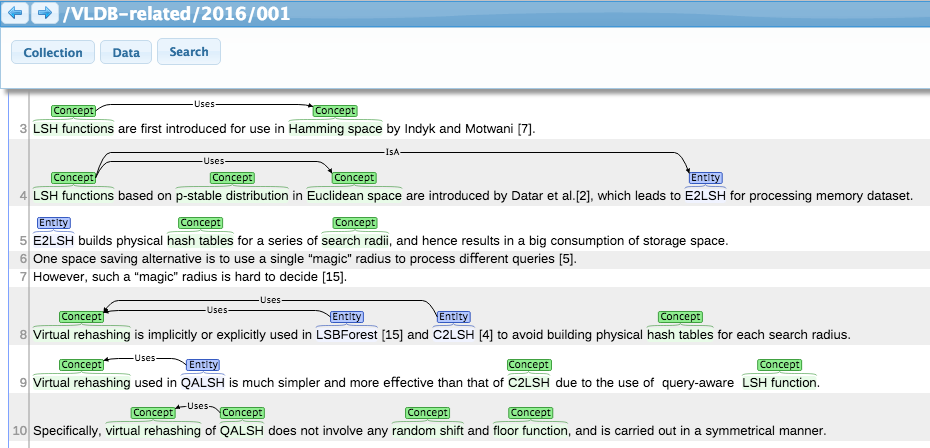
\includegraphics[width=1.0\textwidth]{./images/brat_img}
  \caption[The Brat rapid annotation tool, an online environment for collaborative text annotation.]{The Brat rapid annotation tool, an online environment for collaborative text annotation.}
  \label{fig:brat_img}
\end{figure}


\subsection{Graphviz}
\pdfbookmark{Graphviz}{pdfmark:graphviz}

\begin{figure}[!htbp]
  \centering
    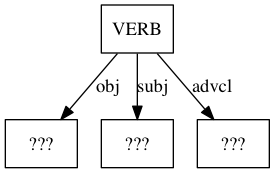
\includegraphics[width=0.4\textwidth]{./images/command-simplified-group-uses-16}
  \caption[The resulting graphic from graphviz.]{The resulting graphic from graphviz from the Figure \ref{fig:dot_lang} DOT specification.}
  \label{fig:dot_img}
\end{figure}

Graphviz\footnote{\url{http://www.graphviz.org/}} is open source graph generation software. It utilises a graph describing language called DOT\footnote{\url{http://www.graphviz.org/doc/info/lang.html}} which is used to generate the graphs using the distributed DOT binary that companions the Graphviz distribution.

In this project, we used its Python wrapper\footnote{\url{https://pypi.python.org/pypi/graphviz}}, which allowed for seamless generation of the DOT file straight from Python objects. As an example, Figure \ref{fig:dot_lang} shows the specification in DOT language that generated the graphic image in Figure \ref{fig:dot_img}

\begin{figure}[!htbp]

\begin{verbatim}
digraph uses {
    node [shape=box]
    1376 [label=VERB]
    1378 [label="???"]
        1376 -> 1378 [label=obj]
    1379 [label="???"]
        1376 -> 1379 [label=subj]
    1377 [label="???"]
        1376 -> 1377 [label=advcl]
}
\end{verbatim}

  \caption[The DOT language.]{The DOT language.}
  \label{fig:dot_lang}
\end{figure}


%
%
% DEVELOPED PROCESS AND PROGRAMS
%
%å

\section{Developed Program}
\pdfbookmark{Developed Program}{pdfmark:devprogram}

Our developed program, namely \emph{corpus\_analysis.py}, accepts as an input a file-system folder of raw text and a verb in its singular third person form, and it then outputs relations of the parameters surrounding that verb in the sentence, aiming for a triplet relation type such as the format: \texttt{Relation ( Argument1 ; Argument2 )}. Figure \ref{fig:html_output} presents the HTML output of the program rendered in a Web Browser.

To some extent, our current approach is similar to that of ClauseIE, in the sense that it completely relies on the dependency parsing tree, but with several key differences:

\begin{itemize}
	\item Due to this verb-centric nature, since the verb is the relation being searched for and is part of the input, our tool tailors the extraction process for each different verb. It does so in the sense that ignores parts of the corpus that does not contain the token we are searching for, as long as there is a sufficiently large corpus to find typical usage of the verbs;
	\item Instead of heuristically determining whether or which PP-attachment, (named \enquote{A} as in the \emph{SVA} sentence type) to be used as object of the verb, we can do it more accurately given that the verb is given as an input. The same is true for \enquote{O} in the \emph{SVO} sentence type;
	\item Also, we extract more than binary relations with an optional typeless argument as ClauseIE did. The output is more in line with these semantic functional analysis of verbs, as in PropBank \cite{Palmer:2005:PBA:1122624.1122628}, or VerNet \cite{Schuler:2005:VBC:1104493};
	\item ClauseIE classifies the sentence being extracted against a list of possible sentences using a decision tree, and then uses this information to decide how to extract the information. In contrast, our method simply applies a sequence of rules in an arbitrary order that attempts to reach out for information in case it is missing in the nodes near the position of the verb in the dependency tree;
	\item Finally, it utilises SpaCy for dependency parsing instead of Stanford CoreNLP. This might affect technological choices as this process could more easily fit into a Python-based pipeline.
\end{itemize}

\begin{figure}[!htbp]
  \centering
    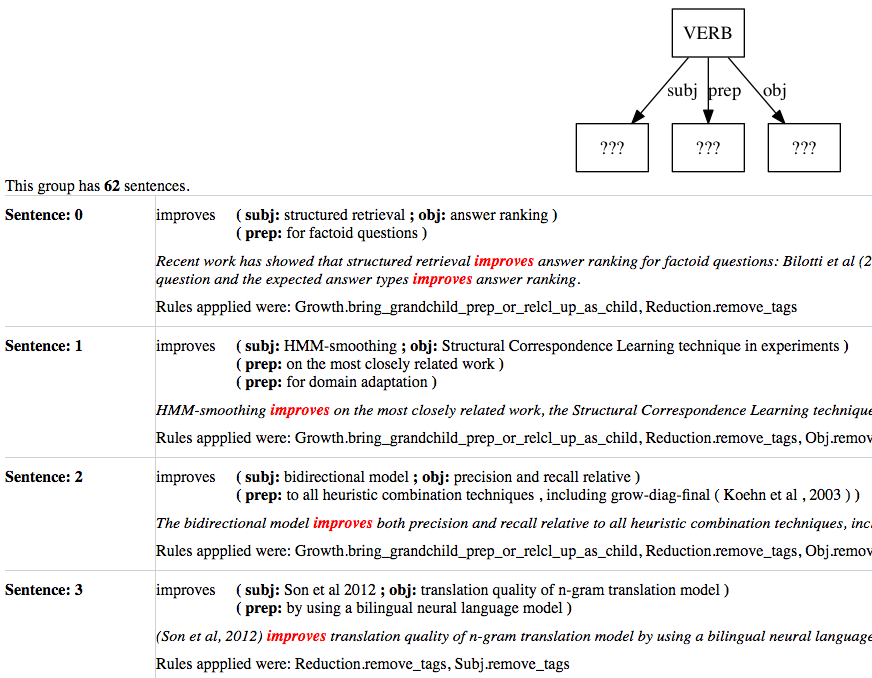
\includegraphics[width=1.0\textwidth]{./images/html_output}
  \caption[The HTML output generated by our program.]{The HTML output generated by our program. Note how it organizes sentences orders by its grouping.}
  \label{fig:html_output}
\end{figure}

Contrary to other tools, such as Stanford OpenIE, we are extracting only explicit information. There is no logical reasoning to better present the information obtained and that is implicit in the text. Moreover, we do not try to match the results of our tool against any knowledge database with the intention to compare what is being learned from the natural text with.

\begin{algorithm}[t]
  \caption{Main loop}\label{main}
  \begin{algorithmic}[1]
    \Procedure{SimplifiedGroup}{$files,verb$}
	
    \For{$sentence, token \ \ \texttt{in} \ \ \Call{GetTokens}{files, verb}$}
       \State $\Call{ApplyGrowthRules}{token}$
       \State $\Call{ApplyReductionRules}{token}$
       \State $\Call{ApplyObjRules}{token}$
       \State $\Call{ApplySubjRules}{token}$
       \State $relations\gets \Call{Extraction}{token}$
       \State $\Call{AddToGroup}{sentence, token, relations}$
    \EndFor
    
    \State $\Call{GenerateOutput}{groups}$
    
    \EndProcedure
  \end{algorithmic}
\end{algorithm}

The main algorithm of our tool is simple in the sense that the goal is to process all entries found in the text containing the verb being looked after. Note that, in Algorithm \ref{main}, \texttt{token} is actually a node in the dependency tree, thus why rules are applied directly into the \texttt{token} variable. The main loop then extract the relations and prepare the grouping presentation. After all this is done, the output is then generated. The goal of the HTML output is for human evaluation and analysis, while the goal of the JSON output is for down-the-line processing by other program.

\begin{algorithm}[t]
  \caption{Iterator to tokens and sentences}\label{get_tokens}
  \begin{algorithmic}[1]
  
    \Procedure{GetTokens}{$files, verb$}
    		\State $finalList\gets \Call{GetFromCache}{files}$
        \If{$\texttt{NOT} \ \ finalList$}
       		\State $list\gets \Call{GetFilesWithVerb}{files, verb}$
       		\State $finalList\gets []$\Comment{Empty list}
    		
           \For{$text \ \ \texttt{in} \ \ list$}
             \State $rawParsed\gets \Call{ParseRawText}{text}$
             \State $spacyParsed\gets \Call{EnglishSpacyModel}{rawParsed}$
             \State $cacheableTreeNode\gets \Call{TranformTree}{spacyParsed}$
             \State $\Call{AppendToList}{finalList, cacheableTreeNode}$
           \EndFor
        
       		\State $\Call{SaveCache}{finalList}$
    		\EndIf
    		
    \State $\texttt{Yield  each} \ \ token, sentence \ \ \texttt{from} \ \ finalList$

    \EndProcedure
    
  \end{algorithmic}
\end{algorithm}

Algorithm \ref{get_tokens} implements a Python iterator\footnote{\url{https://docs.python.org/3.4/reference/expressions.html\#generator-iterator-methods}} using the \texttt{yield} keyword. It starts by attempting to find a copy of the parsed tree already cached for performance purposes. If a cached version exists, it is used instead. Caching was implemented as follows: A cache entry has a key, which combines the verb being searched for and the date in which the input folder containing the raw text was last modified. This means that a cache entry can only be found if the folder was not modified and the verb being searched for now was already searched for before. We had to implement our own tree data structure that mimics the SpaCy data structure since the SpaCy tree was not serializable with Pickle\footnote{\url{https://docs.python.org/3.4/library/pickle.html}}, the Python library responsible for serialization. In line 9 of Algorithm \ref{get_tokens} we can see that the \texttt{cacheableTreeNode} variable is the same as the \texttt{token} variable, which is yielded later on by the function.


\begin{figure}[!htbp]

\begin{verbatim}
u [ a [ b c d]
    e [f [g h] i]
    k 
  ]
}
\end{verbatim}

  \caption[A tree denoted using QTREE.]{A tree denoted using QTREE.}
  \label{fig:qtree_lang}
\end{figure}


Algorithm \ref{generate_representation} depicts the grouping of sentences by representation in a dictionary, which is the Python equivalent to a hash-table. In line 2, one can see the \textsc{GroupQTREERepr} method which, given the token data structure, generated the QTREE \cite{qtree} representation of it for grouping purposes. Note that this is not the full tree, but only a smaller version used for analysis as described in Section \ref{section:grouping}. The QTREE representation was chosen to be the canonical representation of the tree data structure, and is then used as the key of the dictionary. This is the result of a performance optimisation on earlier versions of the tool, which instead compared the tree which already existing entry in a list before deciding if it already existed in it or not. This brings this part of the process asymptotically from $\mathcal{O}(n)$ time to a much faster in practice constant $\mathcal{O}(1)$ time.

\begin{algorithm}[t]
  \caption{Accumulate sentences}\label{generate_representation}
  \begin{algorithmic}[1]
    
    \Procedure{AddToGroup}{$sentence, token, relations$}
    		\State $groupRepr\gets \Call{GroupQTREERepr}{token}$ \Comment{Group representation}
    		\State $\Call{GenerateSentenceImage}{sentence}$
    		\State $\Call{GenerateGroupImage}{groupRepr}$
    		
    		\If{$groupRepr \ \ \texttt{not in} \ \ groups$}
    			\State $\Call{AppendToGroup}{groups, groupRepr}$
    		\EndIf
    		
    		\State $\Call{AppendToGroup}{groups[_{groupRepr}], sentence, relations}$
    		
    \EndProcedure
    
  \end{algorithmic}
\end{algorithm}


In QTREE one uses the square brackets symbol to denote the edges and the hierarchy of the tree in text mode, resulting in a string representation of it. See an example in Figure \ref{fig:qtree_lang}.

Some specific adjustments were added to the procedure \textsc{ParseRawText} (in line 7 of Algorithm \ref{get_tokens}), as follows:
\begin{itemize}
  \item Applies a regular expression to replace all \emph{\enquote{et al.}} strings with an empty string. This is done to improve sentence segmentation in SpaCy which was in several occasions specifically confusing the term with a sentence boundary;
  \item Another small tweak was done in the SpaCy tokenizer as to not split words that contain a dash in the middle, such as \emph{\enquote{data-mining}}. A file called \texttt{infix.txt}\footnote{More precisely, when using virtualenv, it sits in in the following location: \texttt{.env/lib/python3.4/site-packages/spacy/data/en-1.1.0/tokenizer/infix.txt}. Virtualenv is a method of installing Python packages only to the local scope of a project, without affecting the traditional global folder where packages are installed (which affect all Python programs in the computer) - more information about virtualenv can be found at \url{https://virtualenv.pypa.io/en/stable/}.}, which is part of the SpaCy data, contains a set of regular expressions for the tokenizer, and the \texttt{(?<=[a-zA-Z])-(?=[a-zA-z])} responsible for tokenizing words with a dash symbol was then deleted. This change made the tree simpler in some situations by reducing the amount of punctuation nodes;
  \item Removed unicode characters from the output by using Python filters to achieve so;
  \item Added a regular expression to remove citations of the type \emph{\enquote{(Lenat, 1995)}}. This avoids SpaCy breaking these as nodes in the tree and diminishes the chances of misclassifications of the dependencies.
\end{itemize}



%
%
% GROUPING SENTENCE TYPES
%
%

\section{Grouping Sentence Types}
\label{section:grouping}
\pdfbookmark{Grouping Sentence Types}{pdfmark:grouping}

This section further describes the purpose of the \textsc{GroupQTREERepr} method from Algorithm \ref{generate_representation}. The grouping of the sentences was done with the goal to facilitate human local analysis. There are four possibilities for grouping: based on the \emph{verb} node (the original verb in which the relation is being searched for), based on the \emph{subj} node, based on the \emph{obj} node, and based on any other of the optional relations nodes.

\begin{figure}[!htbp]
  \centering
    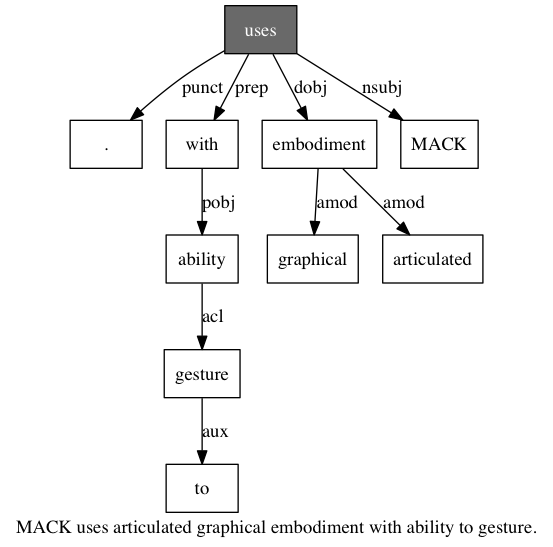
\includegraphics[width=0.6\textwidth]{./images/sentence-91-37}
  \caption[The Graphviz output generated by SpaCy dependency tree.]{The Graphviz output generated by SpaCy dependency tree.}
  \label{fig:tree_output}
\end{figure}

The grouping works as follows. Given the node the grouping is based on, the immediate children are extracted and a new tree is formed only with the node plus its children. For an example, given the sentence \emph{\enquote{MACK uses articulated graphical embodiment with ability to gesture.}}. Suppose we are searching for the \emph{Uses} relation. The dependency tree from SpaCy is generated and presented in Figure \ref{fig:tree_output}. The \texttt{token} being analysed by the algorithm is then the word \emph{uses}, at the top of the tree. The tree has four child nodes, however we disregard the actual child nodes values, and pay attention only to the actual dependencies, or edges values, between \texttt{token} and its children. This results in the summarized version of the tree presented in Figure \ref{fig:group_output_2}. This is the tree that represents this sentence in this grouping.

\begin{figure}[!htbp]
  \centering
    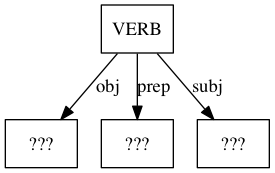
\includegraphics[width=0.4\textwidth]{./images/command-simplified-group-uses-3}
  \caption[The group of the sentence.]{The group of the sentence from Figure \ref{fig:tree_output}.}
  \label{fig:group_output_2}
\end{figure}

Note that the \emph{punct} dependency is missing in the final group, and this is due to the rules applied by Algorithm \ref{main} to this resulting tree as to adjust and improve the grouping. More precisely, we wanted to ignore the \emph{punct} dependency in the group, as it had no observed effect in our analysis of the tree and the location of the \emph{subj}-like and \emph{dobj}-like dependencies we are mostly after. This will be explained further in Section \ref{section:rules}. 

We also used a similar grouping in an attempt to observe the other parameters that are optionally part of the relation, assuming they would be attached to the \texttt{token} node by SpaCy. This would be more in line with efforts such as PropBank \cite{Palmer:2005:PBA:1122624.1122628}, or VerNet \cite{Schuler:2005:VBC:1104493}. A more complex example is the sentence \emph{\enquote{Our work not only improves the CPU efficiency by three orders of magnitude, but also reduces the memory consumption}} which, through the same process, produces the group representation in Figure \ref{fig:group_output_3}.

\begin{figure}[!htbp]
  \centering
    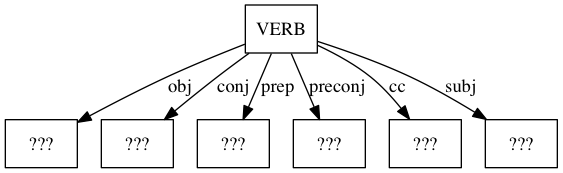
\includegraphics[width=0.6\textwidth]{./images/command-simplified-group-improves-29}
  \caption[A more complex example of sentence grouping.]{A more complex example of sentence grouping.}
  \label{fig:group_output_3}
\end{figure}



%
%
% DEPENDENCY TREE MANIPULATION RULES
%
%

\section{Dependency Tree Manipulation Rules}
\label{section:rules}
\pdfbookmark{Dependency Tree Manipulation Rules}{pdfmark:dependencyrules}

This section further describes the purpose of the rule application methods in the main loop of Algorithm \ref{main}. During the process of obtaining the trees for the searched verb, several rules are applied as to organise the tree in a way that facilitates the extraction method. These rules are applied by four different Python classes: \texttt{Growth}, \texttt{Reduction}, \texttt{Obj}, \texttt{Subj}, in this order. We use a custom annotator to identify which methods of these classes are actual rules to be applied. The rules are applied in the order they appear in these classes. The addition of new rules, in an investigative setting, simply requires the addition of an annotated method in any of these classes.

The \texttt{Growth} and \texttt{Reduction} classes apply the rules from the perspective of the node which represents the verb being looked for, i.e., the method receives the verb as the node to do the analysis on. The \texttt{Growth} class intends to have rules which cause currently unavailable information to be obtained from other parts of the tree, while the \texttt{Reduction} class intends to have rules that remove irrelevant information.

Moreover, in the \texttt{Obj} and \texttt{Subj} classes, the rules are applied on the node that currently represents respectively:

\begin{itemize}
  \item \emph{obj}-like relations: Direct Object (\emph{dobj}); Object of Preposition (\emph{pobj}), Indirect Object (\emph{iobj}); or
  \item \emph{subj}-like relations: Nominal Subject (\emph{nsubj}), Clausal Subject  (\emph{csubj}), Passive Nominal Subject (\emph{nsubjpass}), Passive Clausal Subject (\emph{csubjpass}) \cite{Marneffe08stanfordtyped}.
\end{itemize}

Further describing the tree structure, it is important to note the strong characteristic that every node of the dependency tree can have from \emph{0} to \emph{n} children, however exactly \emph{1} head (or parent) node. For each actual node dependency tree, we also generate a separate tree representation which is used for grouping. In some cases (which will be denoted), these rules apply only in the representation and not to the original tree. This means that, although we want some trees to be grouped together to facilitate analysis, the original version might still be used for the rule extraction.

A final class called \texttt{Extraction} apply a single extraction method which obtains the parts of the relation after all rules above are applied. The extraction method trivially outputs all the child nodes from the node that represents the verb which is the relation being looked for. The rules are defined as follows.

As a baseline example to start with, note the sentence \emph{\enquote{We stress that our method improves a supervised baseline}} where the tree generated by the dependency parser is already \enquote{optimal}, in the sense that the information is ready to be extracted without any tree manipulation. See Figure \ref{fig:no_rule} for the dependency tree. The extracted relation by our tool is \texttt{improves ( our method ; supervised baseline )}, which is basically the text form of the verb sub-trees. Consequently, we list now the rules created for our system to increase its ability to extract information in other \enquote{non-optimal}, more complex trees. 


\begin{figure}[!htbp]

\centering
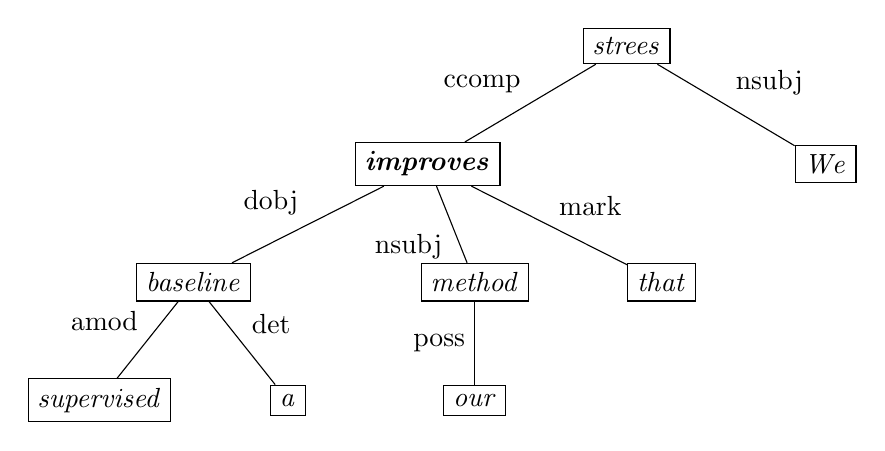
\begin{tikzpicture}[every tree node/.style={draw},
   level distance=1.50cm,sibling distance=1.25cm,
   edge from parent path={(\tikzparentnode) -- (\tikzchildnode)}]
\Tree
[.\textit{strees}
  \edge node[auto=right] {ccomp}; [.\textit{\textbf{improves}}
  		\edge node[auto=right] {dobj}; [.\textit{baseline}
			\edge node[auto=right] {amod}; [.\textit{supervised} ]
			\edge node[auto=left] {det}; [.\textit{a} ]  		
  		]
  		\edge node[auto=right] {nsubj}; [.\textit{method}
			\edge node[auto=right] {poss}; [.\textit{our} ]  		
  		]
  		\edge node[auto=left] {mark}; [.\textit{that} ]  
  ]
	\edge node[auto=left] {nsubj}; [.\textit{We} ]
]
\end{tikzpicture}

\caption[A sentence whose relation can be obtained without tree manipulation.]{A sentence whose relation can be obtained without tree manipulation.}
\label{fig:no_rule}
\end{figure}


\begin{treerule}[\texttt{Growth}]
\label{treerule:rule1}
If the edge to the head node is of the type \emph{relcl} or \emph{ccomp}, and the existing \emph{subj}-like child node does not have the POS tag \emph{NOUN}, \emph{PROPN}, \emph{VERB}, \emph{NUM}, \emph{PRON}, or \emph{X}, replace the \emph{subj}-like child node with the immediate head node. If there is no \emph{subj}-like child node, simply move the head node as to be its \emph{subj}-like child.
\end{treerule}

In Rule \ref{treerule:rule1}, we replace the subject when in a relative clause or clausal complement. In this setting, it is common that the verb does not have a \emph{subj}-like child node, or that it has a non-meaningful one (such as \emph{\enquote{which}}, or \emph{\enquote{that}}). Note how this situation occurs in the sentence \emph{\enquote{Calvin [21] is a distributed main-memory database system that uses a deterministic execution strategy}}, when searching for the \emph{\enquote{uses}} relation. Figure \ref{fig:rule1_before} shows the raw tree from the SpaCy dependency parser, and Figure \ref{fig:rule1_after} shows it after the rule application. The relation extracted in this case is: \texttt{uses	( distributed main-memory database system ; deterministic execution strategy )}.

\begin{figure}[!htbp]
\centering

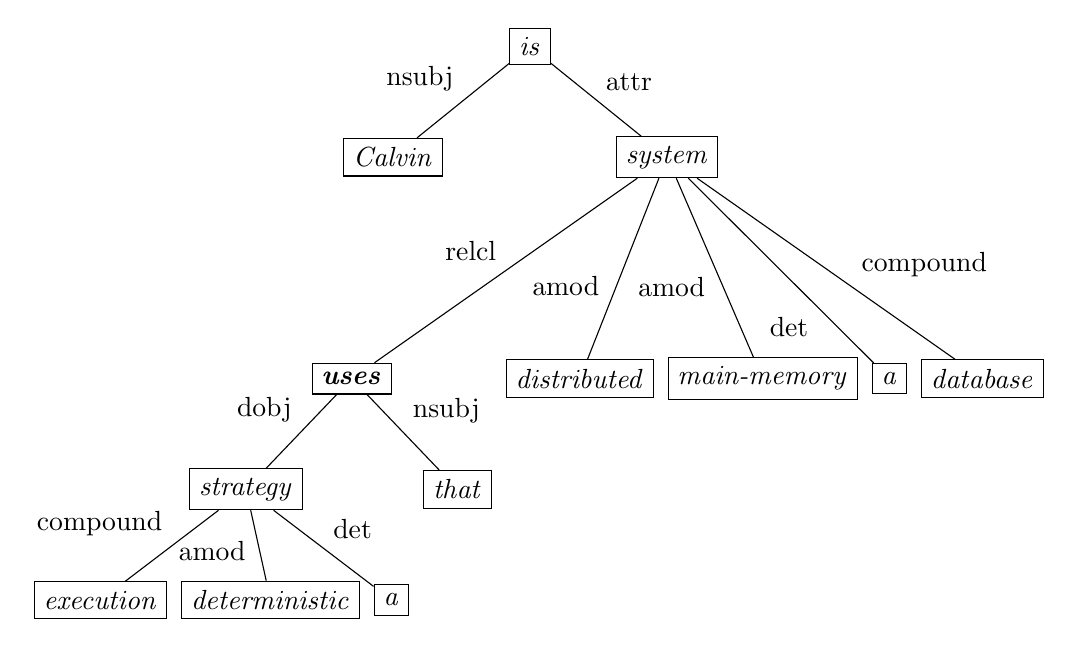
\begin{tikzpicture}[every tree node/.style={draw,align=center},
   level distance=40pt,
   sibling distance=5pt,
   level 1/.style={sibling distance=-150pt},
   level 2/.style={level distance=80pt},
   edge from parent path={(\tikzparentnode) -- (\tikzchildnode)}]
\Tree
[.\textit{is}
  \edge node[auto=right] {nsubj}; [.\textit{Calvin} ]
  \edge node[auto=left] {attr}; [.\textit{system}
	  \edge node[auto=right] {relcl}; [.\textit{\textbf{uses}}
		  \edge node[auto=right] {dobj}; [.\textit{strategy}
			  \edge node[auto=right] {compound}; [.\textit{execution} ]
			  \edge node[auto=right,pos=0.3] {amod}; [.\textit{deterministic} ]
			  \edge node[auto=left] {det}; [.\textit{a} ]
		  ]
		  \edge node[auto=left] {nsubj}; [.\textit{that} ]
	  ]
	  \edge node[auto=right,pos=0.7] {amod}; [.\textit{distributed} ]
	  \edge node[auto=right,pos=0.5] {amod}; [.\textit{main-memory} ]
	  \edge node[auto=right,pos=0.7] {det}; [.\textit{a} ]
	  \edge node[auto=left,pos=0.6] {compound}; [.\textit{database} ]
  ]
]
\end{tikzpicture}

\caption[A sentence that depicts a tree in which the application of Rule \ref{treerule:rule1} is possible (before).]{A sentence that depicts a tree in which the application of Rule \ref{treerule:rule1} is possible (before).}
\label{fig:rule1_before}
\end{figure}


\begin{figure}[!htbp]
\centering

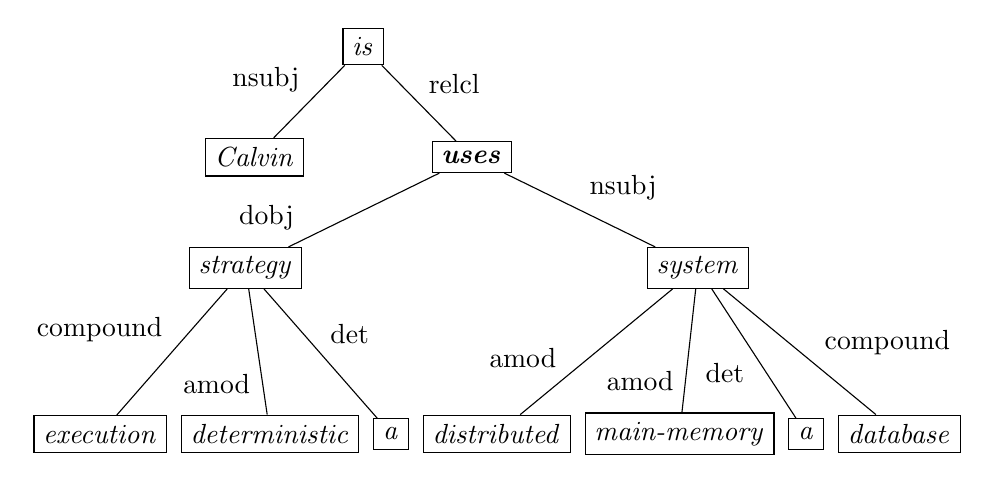
\begin{tikzpicture}[every tree node/.style={draw,align=center},
   level distance=40pt,
   sibling distance=5pt,
   level 1/.style={sibling distance=-100pt},
   level 3/.style={level distance=60pt},
   edge from parent path={(\tikzparentnode) -- (\tikzchildnode)}]
\Tree
[.\textit{is}
  \edge node[auto=right] {nsubj}; [.\textit{Calvin} ]
  \edge node[auto=left] {relcl}; [.\textit{\textbf{uses}}
	  \edge node[auto=right,pos=0.9] {dobj}; [.\textit{strategy}
		  \edge node[auto=right] {compound}; [.\textit{execution} ]
		  \edge node[auto=right,pos=0.6] {amod}; [.\textit{deterministic} ]
		  \edge node[auto=left] {det}; [.\textit{a} ]
	  ]
	  \edge node[auto=left] {nsubj}; [.\textit{system}
		  \edge node[auto=right,pos=0.7] {amod}; [.\textit{distributed} ]
		  \edge node[auto=right,pos=0.9] {amod}; [.\textit{main-memory} ]
		  \edge node[auto=right,pos=0.5] {det}; [.\textit{a} ]
		  \edge node[auto=left,pos=0.6] {compound}; [.\textit{database} ]
    ]
  ]
]
\end{tikzpicture}

\caption[The sentence from Figure \ref{fig:rule_before} after application of Rule \ref{treerule:rule1}.]{The sentence from Figure \ref{fig:rule1_before} after application of Rule \ref{treerule:rule1}.}
\label{fig:rule1_after}
\end{figure}

\begin{treerule}[\texttt{Growth}]
\label{treerule:rule2}
If the current node is part of a \emph{conj} relation through its head edge, and no \emph{subj}-like child node exists, search for a \emph{subj}-like child node in the parent (a sibling node). Recurse in case this is not found and the head edge is again a \emph{conj}.
\end{treerule}

In Rule \ref{treerule:rule2}, we obtain subject from parent if in a conjunct relation. This normally occurs once the parser decides that the relation being searched for is part of a bigger set of relations the subject of the sentence is part of. For an example, note in Figure \ref{fig:rule2_before_after} how the sentence \emph{\enquote{SemTag uses the TAP knowledge base5, and employs}} depicts the subject \emph{\enquote{SemTag}} being further away from the verb \emph{\enquote{employs}}, the relation being searched for. In this case, before the rule application \emph{\enquote{SemTag}} is a sibling node of \emph{\enquote{employs}}, both being child nodes of \emph{\enquote{uses}}.


\begin{figure}[!htbp]
\centering

\begin{minipage}{.5\textwidth}
\centering
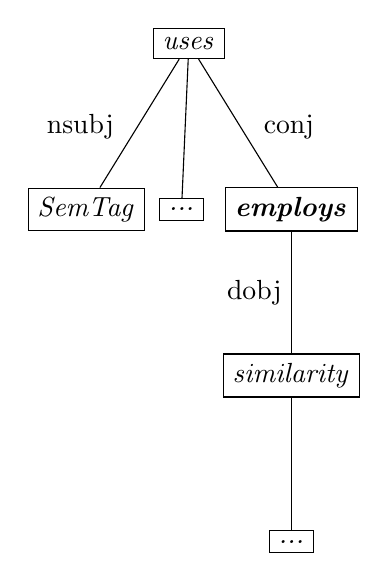
\begin{tikzpicture}[every tree node/.style={draw,align=center},
   level distance=60pt,
   sibling distance=5pt,
   edge from parent path={(\tikzparentnode) -- (\tikzchildnode)}]
\Tree
[.\textit{uses}
  \edge node[auto=right,pos=0.7] {nsubj}; [.\textit{SemTag} ]
  [.\textit{...} ]
  \edge node[auto=left,pos=0.7] {conj}; [.\textit{\textbf{employs}}
	  \edge node[auto=right] {dobj}; [.\textit{similarity}
			[.\textit{...} ]	  
	  ]
  ]
]
\end{tikzpicture}

\end{minipage}%  no empty line here 
\begin{minipage}{.5\textwidth}
\centering
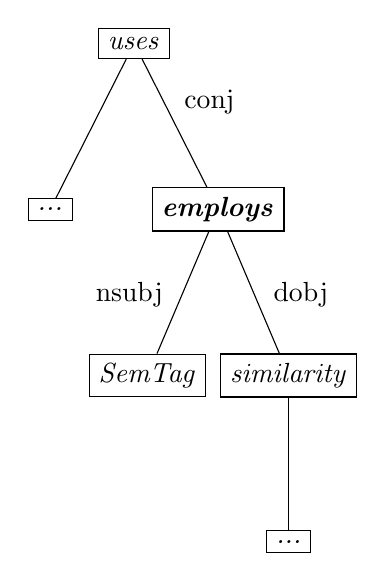
\begin{tikzpicture}[every tree node/.style={draw,align=center},
   level distance=60pt,
   sibling distance=5pt,
   edge from parent path={(\tikzparentnode) -- (\tikzchildnode)}]
\Tree
[.\textit{uses}
  [.\textit{...} ]
  \edge node[auto=left] {conj}; [.\textit{\textbf{employs}}
    \edge node[auto=right,pos=0.7] {nsubj}; [.\textit{SemTag} ]
	  \edge node[auto=left,pos=0.7] {dobj}; [.\textit{similarity}
			[.\textit{...} ]	  
	  ]
  ]
]
\end{tikzpicture}

\end{minipage}
%  no empty line here 

\caption[A partial tree of a sentence that depicts a tree in which the application of Rule \ref{treerule:rule2} is possible (before).]{A partial tree of a sentence that depicts a situation in which the application of Rule \ref{treerule:rule2} is possible (before on the left, and after the application on the right).}
\label{fig:rule2_before_after}
\end{figure}


\begin{treerule}[\texttt{Growth}]
\label{treerule:rule3}
If no \emph{obj}-like child node exists, transform nodes \emph{xcomp} or \emph{ccomp} in a \emph{dobj}. If no \emph{subj}-like child node exists, transform nodes \emph{xcomp} or \emph{ccomp} in a \emph{nsubj}.
\end{treerule}

\begin{treerule}[\texttt{Growth}]
\label{treerule:rule4}
If no \emph{obj}-like child node exists, transform \emph{prep} relation whose preposition word is \emph{\enquote{in}} in a \emph{dobj} node.
\end{treerule}

Rules \ref{treerule:rule3} and \ref{treerule:rule4}, handle further transformations, or edge renaming, on existing child nodes to improve relation extractions. In Rule \ref{treerule:rule3} the clausal complements with both internal or external subjects, which often contain the missing part of a relation are renamed to be the subject of or object of the sentence.

An example for Rule \ref{treerule:rule4} is the partial sentence \emph{\enquote{matrix co-factorization helps to handle multiple aspects of the data and improves in predicting individual decisions}}, when searching for the \emph{\enquote{improves}} relation. Normally, the parser annotates \emph{\enquote{in predicting (...)}} as a sub clause with a \emph{prep} edge relation, however, in this case, this clause does contain the object being improved by the subject.

\begin{treerule}[\texttt{Growth}]
\label{treerule:rule5}
If no \emph{obj}-like child edge exists, a \emph{subj}-like child edge exists, and the head edge is of the \emph{subj}-like type, move the head node as to be its \emph{dobj}-like child.
\end{treerule}

Another rule that does tree manipulation, Rule \ref{treerule:rule5} caters for situations where the relation being searched for is itself found in a \emph{subj}-like edge connected with its head node. Figure \ref{fig:rule5_before_after} notes this rule being applied in the sentence \emph{\enquote{This work uses materialized views to further benefit from commonalities across queries}}, when searching for the \emph{\enquote{uses}} relation.


\begin{figure}[!htbp]
\centering

\begin{minipage}{.5\textwidth}
\centering
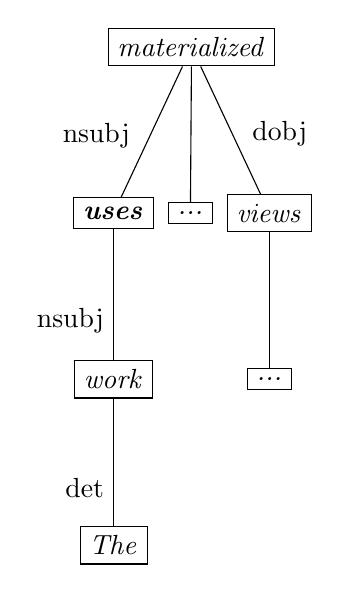
\begin{tikzpicture}[every tree node/.style={draw,align=center},
   level distance=60pt,
   sibling distance=5pt,
   edge from parent path={(\tikzparentnode) -- (\tikzchildnode)}]
\Tree
[.\textit{materialized}
  \edge node[auto=right,pos=0.7] {nsubj}; [.\textit{\textbf{uses}}
    \edge node[auto=right,pos=0.7] {nsubj}; [.\textit{work}
			\edge node[auto=right,pos=0.7] {det}; [.\textit{The} ]    
    ]
  ]
  [.\textit{...} ]
  \edge node[auto=left,pos=0.7] {dobj}; [.\textit{views}
		[.\textit{...} ]  
  ]
]
\end{tikzpicture}

\end{minipage}%  no empty line here 
\begin{minipage}{.5\textwidth}
\centering
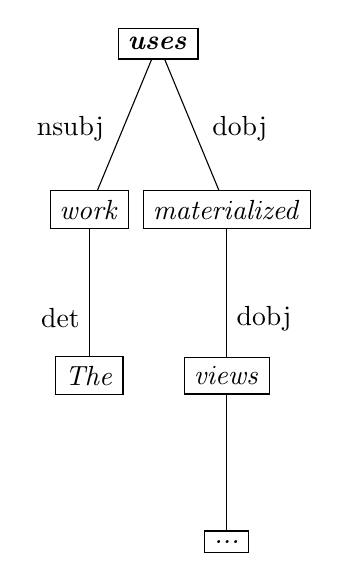
\begin{tikzpicture}[every tree node/.style={draw,align=center},
   level distance=60pt,
   sibling distance=5pt,
   edge from parent path={(\tikzparentnode) -- (\tikzchildnode)}]
\Tree
[.\textit{\textbf{uses}}
  \edge node[auto=right,pos=0.7] {nsubj}; [.\textit{work}
	  \edge node[auto=right,pos=0.7] {det}; [.\textit{The} ]    
  ]
  \edge node[auto=left,pos=0.7] {dobj}; [.\textit{materialized}
  		\edge node[auto=left,pos=0.7] {dobj}; [.\textit{views}
  		  [.\textit{...} ] 
  		]
  ]
]
\end{tikzpicture}

\end{minipage}
%  no empty line here 

\caption[A partial tree of a sentence that depicts a tree in which the application of Rule \ref{treerule:rule5} is possible (before).]{A partial tree of a sentence that depicts a situation in which the application of Rule \ref{treerule:rule5} is possible (before on the left, and after the application on the right).}
\label{fig:rule5_before_after}
\end{figure}



\begin{treerule}[\texttt{Reduction}, representation only]
\label{treerule:rule_reduction1}
For any two child with same incoming edge type, remove the duplicate edge.
\end{treerule}

\begin{treerule}[\texttt{Reduction}]
\label{treerule:rule_reduction2}
Remove tags of type \emph{punct}, \emph{mark}, \emph{\enquote{ }} (empty space), \emph{meta}.
\end{treerule}

\begin{treerule}[\texttt{Reduction}]
\label{treerule:rule_reduction3}
Transform specific edge types of child nodes into a more general version. More specifically, transform all \emph{obj}-like relations into \emph{obj}, all \emph{subj}-like relations into \emph{subj}, and all \emph{mod}-like relations into \emph{mod}.
\end{treerule}

Rule \ref{treerule:rule_reduction1} is the first one we describe of the \texttt{Reduction} type, and together with Rules  \ref{treerule:rule_reduction2} and \ref{treerule:rule_reduction3} serve a main purpose of simplifying the tree representation for grouping and analysis purposes. Rule \ref{treerule:rule_reduction1} removes duplicates only in the representation and causes the analysis of a node with two \emph{prep} child nodes to be the same as a node with only one.

\begin{treerule}[\texttt{Reduction}]
\label{treerule:rule_reduction4}
Merge all \emph{obj}-like relations into one single \emph{obj} node, and all \emph{subj}-like relations into one \emph{subj} node.
\end{treerule}

To describe Rules \ref{treerule:rule_reduction3} and \ref{treerule:rule_subj3}, it is important to note the definition of \emph{mod}-like relations, as per the following:
\begin{itemize}
  \item \emph{mod}-like relations: Noun Phrase Adverbial Modifier (\emph{npadvmod}), Adjectival Modifier (\emph{amod}), Adverbial Modifier (\emph{advmod}), Numeric Modifier (\emph{nummod}), Quantifier Modifier (\emph{quantmod}), Relative Clause Modifier (\emph{rcmod}), Temporal Modifier (\emph{tmod}), Reduced Non-finite Verbal Modifier (\emph{vmod}) \cite{Marneffe08stanfordtyped}.
\end{itemize}

\begin{treerule}[\texttt{Subj} and \texttt{Obj}, representation only]
\label{treerule:rule_subj1}
For any two child with same incoming edge type, remove the duplicate edge.
\end{treerule}

\begin{treerule}[\texttt{Subj} and \texttt{Obj}]
\label{treerule:rule_subj2}
Remove tags of type \emph{det} and \emph{\enquote{ }} (empty space).
\end{treerule}

\begin{treerule}[\texttt{Subj} and \texttt{Obj}]
\label{treerule:rule_subj3}
Transform specific edge types of child nodes into a more general version. More specifically, transform all \emph{obj}-like relations into \emph{obj}, all \emph{subj}-like relations into \emph{subj}, and all \emph{mod}-like relations into \emph{mod}.
\end{treerule}

Rules \ref{treerule:rule_subj1}, \ref{treerule:rule_subj2}, \ref{treerule:rule_subj3} behave similarly to the \texttt{Reduction} rules, but at the \texttt{Subj}, \texttt{Obj} level - these rules intend to facilitate grouping and analysis.

\begin{figure}[!htbp]
\centering

\begin{minipage}{.5\textwidth}
\centering
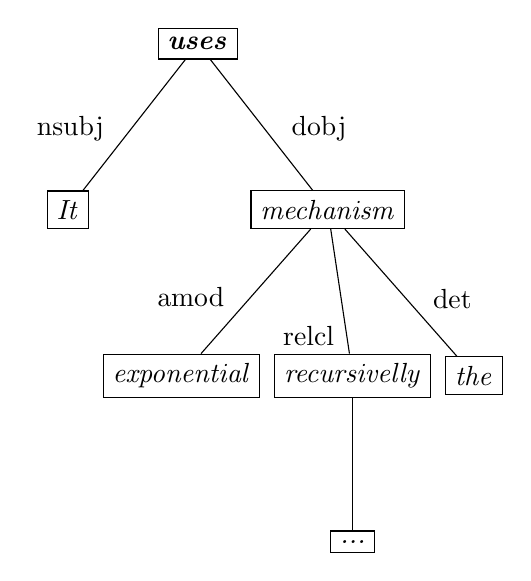
\begin{tikzpicture}[every tree node/.style={draw,align=center},
   level distance=60pt,
   sibling distance=5pt,
   edge from parent path={(\tikzparentnode) -- (\tikzchildnode)}]
\Tree
[.\textit{\textbf{uses}}
  \edge node[auto=right,pos=0.7] {nsubj}; [.\textit{It} ]
  \edge node[auto=left,pos=0.7] {dobj}; [.\textit{mechanism}
			\edge node[auto=right,pos=0.7] {amod}; [.\textit{exponential} ]
			\edge node[auto=right,pos=0.7] {relcl}; [.\textit{recursivelly}
				[.\textit{...} ]
			]
			\edge node[auto=left,pos=0.7] {det}; [.\textit{the} ]
  ]
]
\end{tikzpicture}

\end{minipage}%  no empty line here 
\begin{minipage}{.5\textwidth}
\centering
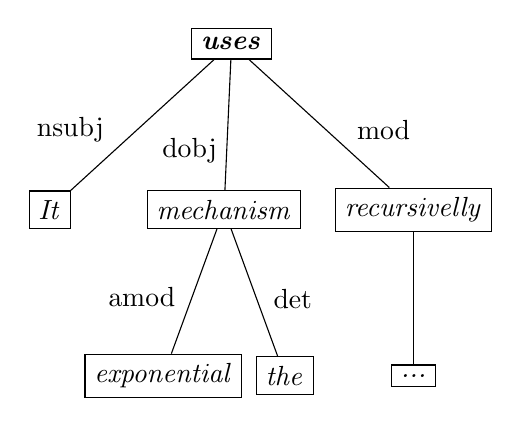
\begin{tikzpicture}[every tree node/.style={draw,align=center},
   level distance=60pt,
   sibling distance=5pt,
   edge from parent path={(\tikzparentnode) -- (\tikzchildnode)}]
\Tree
[.\textit{\textbf{uses}}
  \edge node[auto=right,pos=0.7] {nsubj}; [.\textit{It} ]
  \edge node[auto=right,pos=0.7] {dobj}; [.\textit{mechanism}
			\edge node[auto=right,pos=0.7] {amod}; [.\textit{exponential} ]
			\edge node[auto=left,pos=0.7] {det}; [.\textit{the} ]
  ]
  \edge node[auto=left,pos=0.7] {mod}; [.\textit{recursivelly}
		[.\textit{...} ]
	]
]
\end{tikzpicture}

\end{minipage}
%  no empty line here 

\caption[A partial tree of a sentence that depicts a tree in which the application of Rule \ref{treerule:rule_subj4} is possible (before).]{A partial tree of a sentence that depicts a situation in which the application of Rule \ref{treerule:rule_subj4} is possible (before on the left, and after the application on the right).}
\label{fig:subj_obj_rule4_before_after}
\end{figure}


\begin{table}[!htbp]
  \centering
    \begin{tabular}{ll}
      \textbf{Rule \#}             & \textbf{Python method name} \\
      1
      & Growth.replace\_subj\_if\_dep\_is\_relcl\_or\_ccomp          \\
      2
      & Growth.recurse\_on\_dep\_conj\_if\_no\_subj          \\
      3
      & Growth.transform\_xcomp\_to\_dobj\_or\_sub\_if\_doesnt\_exists          \\
      4
      & Growth.transform\_prep\_in\_to\_dobj          \\
      5
      & Growth.add\_dobj\_if\_dep\_is\_subj          \\
      6
      & Reduction.remove\_duplicates          \\
      7
      & Reduction.remove\_tags          \\
      8
      & Reduction.transform\_tags          \\
      9
      & Reduction.merge\_multiple\_subj\_or\_dobj          \\
      10
      & Obj.remove\_duplicates; Subj.remove\_duplicates          \\
      11
      & Obj.remove\_tags; Subj.remove\_tags          \\
      12
      & Obj.tranform\_tags; Subj.tranform\_tags          \\
      13
      &\specialcell{Obj.bring\_grandchild\_prep\_or\_relcl\_up\_as\_child;
       \\
       Subj.bring\_grandchild\_prep\_or\_relcl\_up\_as\_child}          \\
    \end{tabular}
  \caption[Rules from this document and the Python method names.]{Rules from this document and the Python method names.}
  \label{tab:rules_from_python}
\end{table}


Furthermore, we observed that, in several situations, the subject or object sentences were too long, mainly due to containing extra information beyond the subject/object concept definition. With information extraction, it is reasonable to assume that the tool should return the information as granular as possible, while still maintaining the possibility for the user to use extra context if needed. In an attempt to alleviate this situation, Rule \ref{treerule:rule_subj4} was created.

Figure \ref{fig:subj_obj_rule4_before_after} shows the modification done by Rule \ref{treerule:rule_subj4} in the sentence \emph{\enquote{It uses the exponential mechanism to recursively bisect each interval into subintervals}}, when searching for the \emph{\enquote{uses}} relation. The relation extracted in this case has an extra parameter \emph{mod}: \texttt{	uses	( subj: It ; obj: exponential mechanism ; mod: to recursively bisect each interval into subintervals )}.

\begin{treerule}[\texttt{Subj} and \texttt{Obj}]
\label{treerule:rule_subj4}
Search for the sub-tree rooted by the current node being analysed (either \emph{subj}-like or a \emph{obj}-like) for certain types of nodes and then split the sub-tree in the following way: the found node is removed from the current sub-tree, and moved to be a child node (sub-tree) of the node that represents the relation (the verb). The node that represents the relation is the head (parent) of the current node being analysed. This rule also renames the node as per the below:
	\begin{itemize}
	  \item \emph{relcl}, \emph{acl}, \emph{advcl} with any token: split and rename to  \emph{mod}.
	  \item \emph{prep} with tokens \emph{\enquote{by}}, \emph{\enquote{to}}, \emph{\enquote{for}}, \emph{\enquote{with}}, \emph{\enquote{whereby}}: split and rename to \emph{prep}.
	\end{itemize}
\end{treerule}


In the HTML output, the tool presents the Python method name of the rules applied to a given sentence. Table \ref{tab:rules_from_python} presents the relation between the rules in this document, and their Python method names.

Finally, after continuous revision, some rules were adjusted to, by omission, also cater for a certain number of cases such as:
	\begin{itemize}
	  \item Appositional modifier: once an apposition is found attached to a subject through an \emph{appos} edge, this will be output in the output as part of the relation.
	  \item Punctuation: it is in general also added to the output given, in this corpus, an excess of situations where square brackets or symbols are used to point to extra information around a concept, such as in a references. 
	\end{itemize}



%
%
% RESULTS
%
%

\chapter{Results}
\label{chapter:results}
\pdfbookmark{Results}{pdfmark:results}

This section describes the experiments and comparisons done of this tool with similar existing ones. To prepare for the experiment, we modified the HTML output to:
	\begin{itemize}
	  \item Include the output of three other similar tools: Stanford OpenIE \cite{angeli-johnsonpremkumar-manning:2015:ACL-IJCNLP}, Max Planck Institute ClauseIE \cite{DelCorro:2013:CCO:2488388.2488420}, AllenAI OpenIE \cite{Etzioni:2011:OIE:2283396.2283398}.
	  \item Modified the program to be able to generate a CSV output so evaluation is possible through normal spreadsheet software.
	\end{itemize}


\section{Experiments}
\pdfbookmark{Experiments}{pdfmark:experiments}

We used SpaCy to segment sentences containing selected words and input the relevant sentences through each system. The output was then evaluated by human in the following way below. Note that there were no points added for the optional parts of a relation.

\begin{itemize}
  \item If \emph{subj} and \emph{obj} are correct, the extractor gets 10 points.
  \item If \emph{subj} or \emph{obj} are correct, but not both, the extractor gets 5 points.
  \item If none \emph{subj} and \emph{obj} are correct, the extractor gets 0 points.
\end{itemize}

\begin{figure}[!htbp]
  \centering
    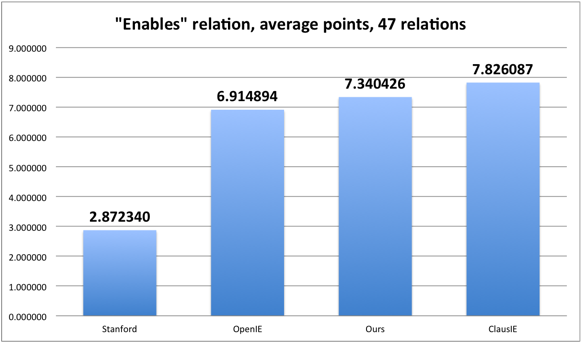
\includegraphics[width=0.8\textwidth]{./images/image001}
  \caption[Results for the \emph{\enquote{enables}} relation.]{Results for the \emph{\enquote{enables}} relation.}
  \label{fig:result_enables}
\end{figure}

\begin{figure}[!htbp]
  \centering
    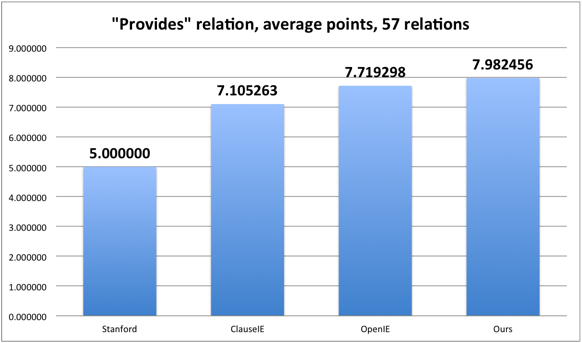
\includegraphics[width=0.8\textwidth]{./images/image002}
  \caption[Results for the \emph{\enquote{provides}} relation.]{Results for the \emph{\enquote{provides}} relation.}
  \label{fig:result_provides}
\end{figure}

Evaluations were done by 2 human specialists. Both Figures \ref{fig:result_enables} and \ref{fig:result_provides} shows the evaluation done by evaluator 1, and promising results from our tool. In the \emph{\enquote{provides}} relation our tool had the best results for this evaluator. These figures are based on the counts form Tables \ref{tab:evaluation_count_provides} and \ref{tab:evaluation_count_enables}.


\begin{table}[!htbp]
  \centering
    \begin{tabular}{|m{2cm}|m{2cm}|m{2cm}|m{2cm}|}
%    \begin{tabular}{m{1cm} m m m}
\hline

 & \textbf{Incorrect} & \textbf{Partial} & \textbf{Correct} \\
\hline

\textbf{Ours}  & 0 & 23 & 34 \\
\hline

\textbf{Stanford}  & 25 & 7 & 25 \\
\hline

\textbf{OpenIE}  & 4 & 18 & 35 \\
\hline

\textbf{ClauseIE}  & 5 & 23 & 29 \\
\hline
    \end{tabular}
  \caption[Evaluation count from evaluator 1 for the \emph{\enquote{provides}} relation.]{Evaluation count from evaluator 1 for the \emph{\enquote{provides}} relation.}
  \label{tab:evaluation_count_provides}
\end{table}



\begin{table}[!htbp]
  \centering
    \begin{tabular}{|m{2cm}|m{2cm}|m{2cm}|m{2cm}|}
%    \begin{tabular}{m{1cm} m m m}
\hline

 & \textbf{Incorrect} & \textbf{Partial} & \textbf{Correct} \\
\hline

\textbf{Ours}  & 0 & 25 & 22 \\
\hline

\textbf{Stanford}  & 28 & 11 & 8 \\
\hline

\textbf{OpenIE}  & 4 & 21 & 22 \\
\hline

\textbf{ClauseIE}  & 1 & 19 & 27 \\
\hline
    \end{tabular}
  \caption[Evaluation count from evaluator 1 for the \emph{\enquote{enables}} relation.]{Evaluation count from evaluator 1 for the \emph{\enquote{enables}} relation.}
  \label{tab:evaluation_count_enables}
\end{table}

For the \emph{\enquote{provides}} relation there is data available from 2 different evaluators. In this case, it is possible to calculate the Kappa measures for the results of the tools, which provides more insights on how the evaluators agree to each other. Tables \ref{tab:comparison_results_evaluators}, \ref{tab:comparison_results_evaluators_stanford}, \ref{tab:comparison_results_evaluators_allenai}, and \ref{tab:comparison_results_evaluators_clauseie} show the agreement of the evaluators across the tools in the format of a confusion matrix. This results in Kappa measures of 41.27\% for our tool, 73.49\% for the Stanford OpenIE tool, 36.81\% for the AllenAI OpenIE tool, and 48.89\% for Max Planck Institute ClauseIE tool.

We believe that these low agreement measures show how difficult it is to standardize the expert evaluation of the understand of what is correctness in Open Information Extraction. Even in this constrained domain (papers from the database area), with experts in this area doing the evaluation, different opinions on what would be the correct extraction emerge, causing differences in the evaluation. The higher agreement number for the Stanford OpenIE extractor comes from the high number of completely incorrect results yielded by the tool.

Another room for disagreement comes from the fact that, while our tool yields only one result, all other Open Information Extraction tools yield multiple relations. Evaluators might then pick different results as the correct one, given the various options in output relations.

\begin{table}[!htbp]
  \centering
\begin{tabular}{l|l|c|c|c|c}
\multicolumn{2}{c}{}&\multicolumn{3}{c}{Evaluator 1}&\\
\cline{3-5}
\multicolumn{2}{c|}{}&Incorrect&Partial&Correct&\multicolumn{1}{c}{Total}\\
\cline{2-5}
\multirow{2}{*}{Evaluator 2}& Incorrect & 0 & 6 & 0 & 6 \\
\cline{2-5}
& Partial & 0 & 5 & 6 & 11 \\
\cline{2-5}
& Correct & 0 & 12 & 28 & 40 \\
\cline{2-5}
\multicolumn{1}{c}{} & \multicolumn{1}{c}{Total} & \multicolumn{1}{c}{0} & \multicolumn{1}{c}{23} & \multicolumn{1}{c}{34} & 57 \\
\end{tabular}

  \caption[Comparison between evaluators for the results of our tool.]{Comparison between evaluators for the results of our tool, based on the \emph{\enquote{provides}} relation.}
  \label{tab:comparison_results_evaluators}
\end{table}


\begin{table}[!htbp]
  \centering
\begin{tabular}{l|l|c|c|c|c}
\multicolumn{2}{c}{}&\multicolumn{3}{c}{Evaluator 1}&\\
\cline{3-5}
\multicolumn{2}{c|}{}&Incorrect&Partial&Correct&\multicolumn{1}{c}{Total}\\
\cline{2-5}
\multirow{2}{*}{Evaluator 2}& Incorrect & 25 & 2 & 1 & 28 \\
\cline{2-5}
& Partial & 0 & 5 & 9 & 14 \\
\cline{2-5}
& Correct & 0 & 0 & 15 & 15 \\
\cline{2-5}
\multicolumn{1}{c}{} & \multicolumn{1}{c}{Total} & \multicolumn{1}{c}{25} & \multicolumn{1}{c}{7} & \multicolumn{1}{c}{25} & 57 \\
\end{tabular}

  \caption[Comparison between evaluators for the results of Stanford OpenIE tool.]{Comparison between evaluators for the results of Stanford OpenIE tool, based on the \emph{\enquote{provides}} relation.}
  \label{tab:comparison_results_evaluators_stanford}
\end{table}


\begin{table}[!htbp]
  \centering
\begin{tabular}{l|l|c|c|c|c}
\multicolumn{2}{c}{}&\multicolumn{3}{c}{Evaluator 1}&\\
\cline{3-5}
\multicolumn{2}{c|}{}&Incorrect&Partial&Correct&\multicolumn{1}{c}{Total}\\
\cline{2-5}
\multirow{2}{*}{Evaluator 2}& Incorrect & 2 & 2 & 0 & 5 \\
\cline{2-5}
& Partial & 0 & 4 & 11 & 15 \\
\cline{2-5}
& Correct & 1 & 12 & 24 & 37 \\
\cline{2-5}
\multicolumn{1}{c}{} & \multicolumn{1}{c}{Total} & \multicolumn{1}{c}{4} & \multicolumn{1}{c}{18} & \multicolumn{1}{c}{35} & 57 \\
\end{tabular}

  \caption[Comparison between evaluators for the results of AllenAI OpenIE tool.]{Comparison between evaluators for the results of AllenAI OpenIE tool, based on the \emph{\enquote{provides}} relation.}
  \label{tab:comparison_results_evaluators_allenai}
\end{table}


\begin{table}[!htbp]
  \centering
\begin{tabular}{l|l|c|c|c|c}
\multicolumn{2}{c}{}&\multicolumn{3}{c}{Evaluator 1}&\\
\cline{3-5}
\multicolumn{2}{c|}{}&Incorrect&Partial&Correct&\multicolumn{1}{c}{Total}\\
\cline{2-5}
\multirow{2}{*}{Evaluator 2}& Incorrect & 5 & 4 & 0 & 9 \\
\cline{2-5}
& Partial & 0 & 4 & 3 & 7 \\
\cline{2-5}
& Correct & 1 & 15 & 26 & 41 \\
\cline{2-5}
\multicolumn{1}{c}{} & \multicolumn{1}{c}{Total} & \multicolumn{1}{c}{5} & \multicolumn{1}{c}{23} & \multicolumn{1}{c}{29} & 57 \\
\end{tabular}

  \caption[Comparison between evaluators for the results of Max Planck Institute ClauseIE tool.]{Comparison between evaluators for the results of Max Planck Institute ClauseIE tool, based on the \emph{\enquote{provides}} relation.}
  \label{tab:comparison_results_evaluators_clauseie}
\end{table}

\section{Cases Analysis}
\label{section:cases}
\pdfbookmark{Cases Analysis}{pdfmark:cases}

This section presents some comparisons of outputs from our tool and ClauseIE.

Given the sentence \emph{\enquote{Crowdsourcing provides a new problem-solving paradigm [3], [21], which has been blended into several research communities, including database and data mining.}}, our tool extracts the relation \texttt{provides	( subj: Crowdsourcing ; obj: a new problem-solving paradigm [ 3 )} with the optional parameter \texttt{( dep: [ 21 ] , which has been blended into several research communities , including database and data mining )}. While Stanford OpenIE extracts no results, and ClauseIE fails to extract any \emph{\enquote{provides}} relation, AllenAI OpenIE extracts the relation but with a very long \emph{obj} that contains the entire sentence starting from \emph{\enquote{a new problem-...}}. This was a situation where the evaluators considered the results of our tool correct, while all others were at most partially correct.

Another similar situation is depicted in Figure \ref{fig:our_tool_success}, which is the actual output of our tool. Note the extracted values at the top, in comparison to the other tools. In this instance the evaluators observed that the Stanford OpenIE tool also yielded a correct result.

\begin{figure}[!htbp]
  \centering
    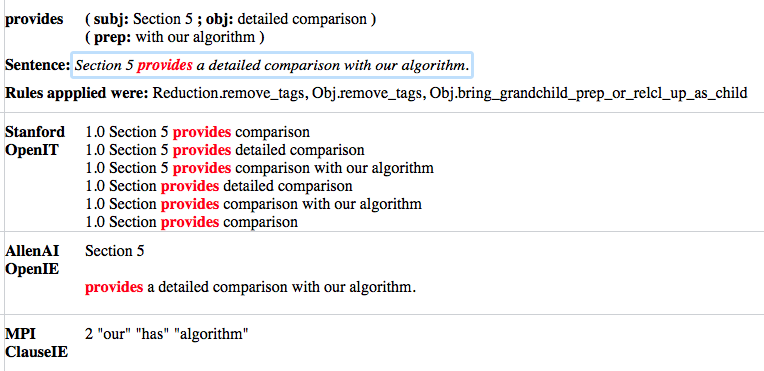
\includegraphics[width=1.0\textwidth]{./images/ours-vs-clauseie}
  \caption[In this example again, our tool is successful in extract the result.]{In this example again, our tool is successful in extract the result.}
  \label{fig:our_tool_success}
\end{figure}

An important point is how reliable our tool is on the correctness of the dependency tree. Figure \ref{fig:our_tool_comparison2} shows a situation where SpaCy mislabels the Part-of-Speech tag of the word \emph{\enquote{set}} in sentence \emph{\enquote{more advantages over a linear result set that are not highlighted in these evaluations}} as a \emph{verb} instead of a \emph{noun} (as it talks about a \emph{\enquote{result set}}). Because of this error, Rule \ref{treerule:rule_subj4} is triggered, causing an incorrect extraction (Figure \ref{fig:our_tool_output_sentence}).


\begin{figure}[!htbp]
  \centering
    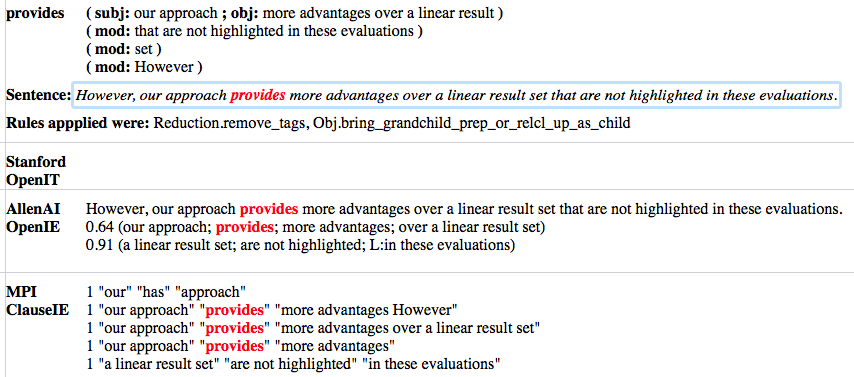
\includegraphics[width=1.0\textwidth]{./images/ours-vs-clauseie-2}
  \caption[In this example, the dependency tree returned by SpaCy is incorrect.]{In this example, the dependency tree returned by SpaCy is incorrect and the rules from our tool cause an incorrect output to be returned.}
  \label{fig:our_tool_comparison2}
\end{figure}


\begin{figure}[!htbp]
  \centering
    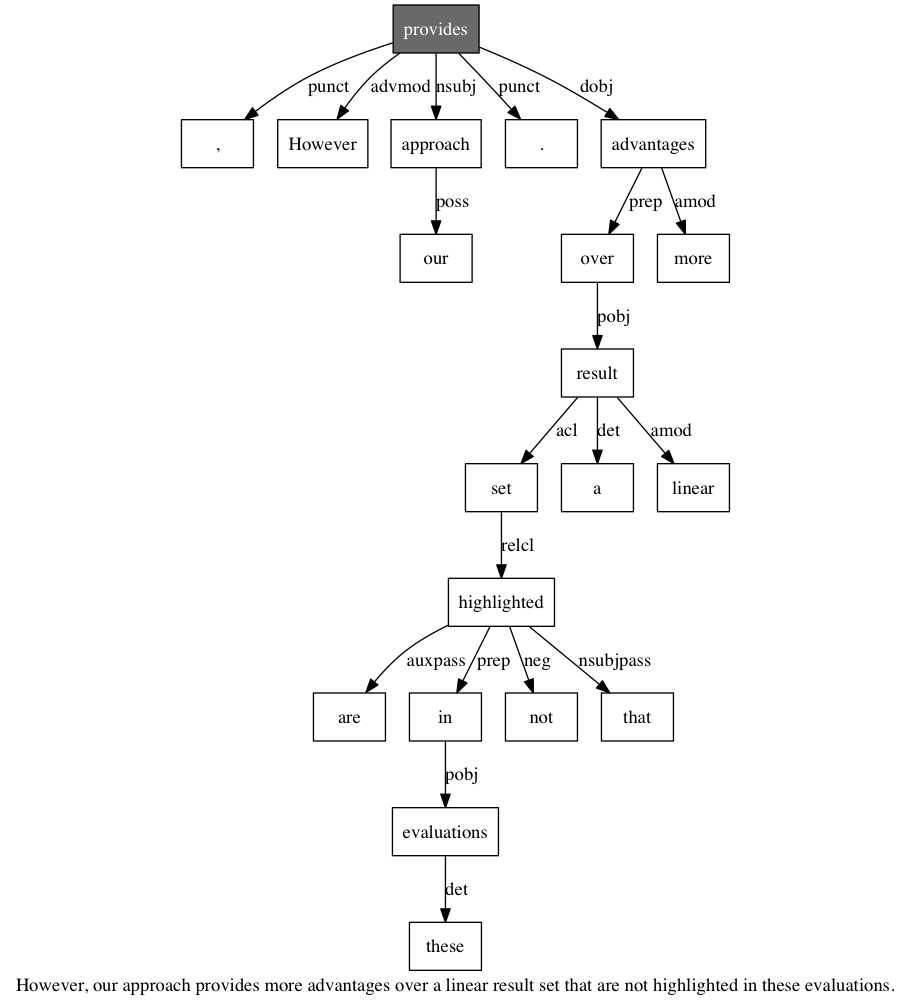
\includegraphics[width=1.0\textwidth]{./images/sentence-164-3}
  \caption[SpaCy's dependency tree.]{SpaCy's dependency tree. Since \emph{\enquote{set}} is wrongly believed to be a verb in this case, it then receives an \emph{acl} dependency label on the edge, triggering Rule \ref{treerule:rule_subj4}. This graph was created by Graphviz also as part of the output of our tool.}
  \label{fig:our_tool_output_sentence}
\end{figure}


\begin{figure}[!htbp]
  \centering
    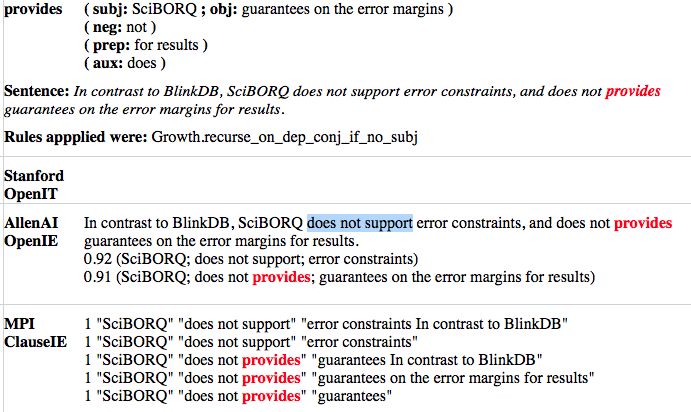
\includegraphics[width=1.0\textwidth]{./images/our-vs-clauseie-3}
  \caption[In this case our tool removes all notions of negation, again yielding an incorrect output.]{In this case our tool removes all notions of negation, again yielding an incorrect output.}
  \label{fig:our_tool_comparison3}
\end{figure}

ClauseIE and AllenAI OpenIE results also retain a notion of negation, while our tool fails to do so. Note that in Figure \ref{fig:our_tool_comparison3} the example shows this behaviour from the output of our tool. Note how in Figure \ref{fig:our_tool_output_sentence2} the dependency tree contains information regarding the negation, however we have no rules that can use this information.

\begin{figure}[!htbp]
  \centering
    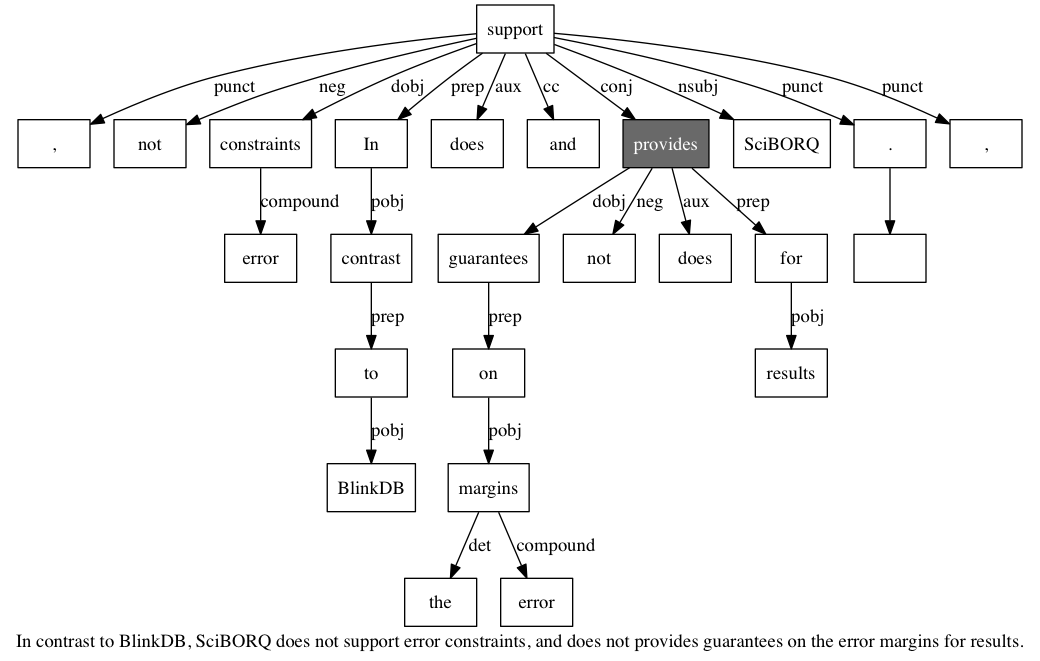
\includegraphics[width=1.0\textwidth]{./images/sentence-4310-6}
  \caption[SpaCy's dependency tree with negation.]{SpaCy's dependency tree correctly provides the negative relations, but our rules fail to use them. This graph was created by Graphviz also as part of the output of our tool.}
  \label{fig:our_tool_output_sentence2}
\end{figure}

The full output of the comparison between the tools contains further examples and nuances, showing the complexity of the problem.


\section{Observed Limits}
\label{section:observations}
\pdfbookmark{Observed Limits}{pdfmark:limits}

We observed that in some cases there are limits on the decision process done by this tool, where the linguistic syntactical information from the text might not be enough, or further semantic knowledge might be needed. Note, for an example, the sentence \emph{\enquote{SemTag uses the TAP knowledge base5 , and employs the cosine similarity with TF-IDF weighting scheme to compute the match degree between a mention and an entity, achieving an accuracy of around 82\%}}. As a result it has the following main structure, mainly due to Rule \ref{treerule:rule_subj4}:
	\begin{itemize}
	  \item \emph{obj}: \emph{\enquote{SemTag}}
	  \item \emph{sub}: \emph{\enquote{cosine similarity}}
	  \item \emph{prep}: \emph{\enquote{with TF-IDF weighting scheme, achieving an accuracy of around 82\%}}
	\end{itemize}

In this domain, \emph{\enquote{cosine similarity with TF-IDF weighting scheme}} would represent a single concept instead, since it is a specific type of \emph{\enquote{cosine similarity}}, contrary to what was the output of the rule. One then observes that, for improved correctness Rule \ref{treerule:rule_subj4} should rely on more information and apply reasoning in order to break the sub-tree more appropriately.

Moreover, it was also possible to note the incapacity of the rules to be applied together, or chained, as to output the correct answers. Note, for an example, the sentence \emph{\enquote{LSD is an extensible framework, which employs several schema-based matchers}}. A new rule could be developed and named Rule A, which processes the \emph{\enquote{is}} relation and follows the \emph{attr} edge as to get the definition for the proper noun \emph{\enquote{LSD}} in this case (Figure \ref{fig:chaining_example}). At this moment, this rule would then yield the relation \texttt{is ( LSD ; an extensible framework )}. Suppose now the \emph{\enquote{employs}} relation is the one actually being searched for. Observing the dependency tree, one could see that Rule \ref{treerule:rule1} would be triggered and cause the head node to be moved and replace the existing \emph{nsubj} child node, yielding \texttt{employs	( extensible framework ; several schema-based matchers )}. At this point, the ability to chain both these rules would yield a more complete relation \texttt{employs	( LSD ; several schema-based matchers )} since the system would already know what \emph{\enquote{LSD}} actually is. In addition, another challenge would be how to have the tool being capable of this decision: when to chain rules, or when knowing that the current result is already optimal.


\begin{figure}[!htbp]

\centering
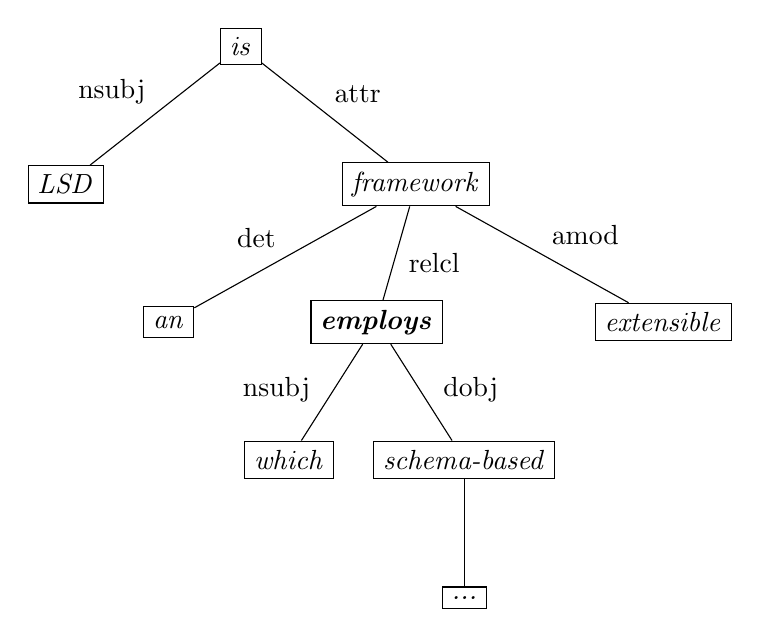
\begin{tikzpicture}[every tree node/.style={draw},
   level distance=1.75cm,sibling distance=0.5cm,
   edge from parent path={(\tikzparentnode) -- (\tikzchildnode)}]
\Tree
[
.\textit{is}
  \edge node[auto=right] {nsubj}; [.\textit{LSD} ]
  \edge node[auto=left] {attr}; [.\textit{framework}
  		\edge node[auto=right] {det}; [.\textit{an} ]
  		\edge node[auto=left,pos=0.4] {relcl}; [.\textit{\textbf{employs}}
  			\edge node[auto=right,pos=0.7] {nsubj}; [.\textit{which} ]
  			\edge node[auto=left,pos=0.7] {dobj}; [.\textit{schema-based}
				[.\textit{...} ]
  			]
  		]
  		\edge node[auto=left] {amod}; [.\textit{extensible} ]
]
]
\end{tikzpicture}

\caption[A sentence that could benefit from rule chaining.]{A sentence that could benefit from rule chaining.}
\label{fig:chaining_example}
\end{figure}

Another observation comes from the simplicity of the \texttt{Extraction} class. In certain situations, multiple relations could have been extracted instead of one. The first case can be seen in sentence \emph{\enquote{As PAS analysis widely employs global and sentence-wide features, it is computationally expensive to integrate}} which in the current tool yields the relation \texttt{employs	( PAS analysis ; global and sentence-wide features )}. A more advanced \texttt{Extraction} rule could attempt to yield two relations instead:
\begin{itemize}
	\item \texttt{employs	( PAS analysis ; global features )}; and
	\item \texttt{employs	( PAS analysis ; sentence-wide features )}.
\end{itemize}

The challenge then sits on deciding when to yield multiple sentences, and what are the tokens that compose them. Note that, in this case, we made the non-trivial decision to repeat the token \emph{\enquote{features}} in both relations.

The second case being, as previously mentioned, regarding the \emph{appos} edge, or appositional modifier. This appears in situations such as in the sentence \emph{\enquote{A similar technique, LightLDA, employs cycle-based Metropolis Hastings mixing}}. While our tool yields one relation \texttt{employs	( similar technique LightLDA ; cycle-based Metropolis Hastings mixing )}, a more advanced \texttt{Extraction} rule could attempt to yield two relations instead:
\begin{itemize}
	\item \texttt{employs	( similar technique ; cycle-based Metropolis Hastings mixing )}; and
	\item \texttt{employs	( LightLDA ; cycle-based Metropolis Hastings mixing )}.
\end{itemize}

Another class of errors observed was when the \emph{obj} contains an intermediate token like \emph{\enquote{us}}. Note, for an example, the sentence \emph{\enquote{Modeling the positions of moving objects as functions of time not only enables us to make tentative future predictions}}. While the expected extraction is \texttt{enables	( Modeling the positions of moving objects as functions of time ; us to make tentative future predictions )}, the system outputs \texttt{enables	( Modeling the positions of moving objects as functions of time ; us )}. This could be resolved by further rules that act on the \emph{obj} replacing the token \emph{\enquote{us}} with the content of the \emph{xcomp} relation where the content of the expected \emph{obj} normally is in these cases and then manipulating the tree accordingly.

Sentence complexity also plays a part in causing errors. Note this sentence: \emph{\enquote{Doing so enables SECOA to securely answer not only all aggregates in [11] without any false positives or false negatives, but also many other aggregates (such as Max, Top- k , Frequent Items, Popular Items) that proof sketches cannot deal with at all.}}. The facts are posed in a format where the sentence structure is more complex (\emph{... not only X ... but also Y}), and there are no rules capable of extracting the information in this format. The extraction is then the follow incomplete fact \texttt{enables	( Doing so ; SECOA )}.

In several other situations, we tracked the error to be due to the dependency tree being incorrect from SpaCy, which was reported as a bug in the project's github page \footnote{\url{https://github.com/explosion/spaCy/issues/480}}. In another category of errors, the problem is due to the data quality problem - the source data (i.e., sentence) is incorrect. This is either due to errors early on in the PDF-to-text extraction process, or issues in SpaCy's segmentation step.


%
%
% CONCLUSION AND FUTURE WORK
%
%


\chapter{Conclusion and Future Work}
\label{chapter:conclusion}
\pdfbookmark{Conclusion and Future Work}{pdfmark:conclusion}

The maturity and fast-pacing on current development of NLP algorithms and frameworks is very positive and provides advanced linguistic information for tackling problems such as information extraction. We observed that the developed tool was reasonably successful, but as the previous section notes that are room for future work on improving the details of its operation.

The addition of semantic information for reasoning in certain rules application would certainly improve the ability of the system to better decide what to do in certain situations, it is unclear however at this point how this would be done. The entities that are part of the relations would benefit from a good disambiguation system and the development of canonical representations of them.

Extra meta-data from the papers, and the entirety of the paper itself, could start being considered. With this one could attempt to answers questions such as:
	\begin{itemize}
	  \item Research relations through time. You could have, e.g., certain historical insights into which algorithm was more popular for a certain task during certain periods;
	  \item Explore coreference resolution more deeply, not only within a paper but across papers and the references between them;
	  \item Events, or introductions of new algorithms or concepts in certain years and how it changes further outputs;
	  \item Building and using a database of the extracted concepts and the relations between them (Knowledge Graph).
	\end{itemize}

Moreover, as future work, one could address the issues described here in Sections \ref{section:cases} and \ref{section:observations} by strengthening the rules for the remaining cases the tool is currently failing. Another issue observed often is the need for a more refined intra-sentence distance evaluation by, for an example, using Stanford's Coreference Resolution output to resolve pronouns into the actual concepts or entities for a more complete relation output.


\backmatter

\printbibliography

\appendix

\end{document}